\documentclass[11pt]{report}

% === Tiếng Việt
\usepackage[utf8]{vietnam}
\usepackage[vietnamese]{babel}
\usepackage{blindtext}

% ===== Thông tin
\title{HỆ THỐNG TẠO VÀ LIÊN KẾT SÀN THƯƠNG MẠI ĐIỆN TỬ CHO NHÀ SẢN XUẤT VÀ CỬA HÀNG}
\author{Trần Ngọc Huy}
\date{Đà Nẵng, Ngày 1 tháng 7 năm 2022}

\newcommand{\advisor}{TS. Lê Thị Mỹ Hạnh}
\newcommand{\msv}{102180208}
\newcommand{\myclass}{18TCLC\_DT3}

% ===== Căn chỉnh lề
\usepackage[
	% >>> Page layout: cỡ giấy A4; lề trái: 3cm, lề phải: 2cm, lề trên: 2,5cm, lề dưới: 2,5cm;
	a4paper,
	left=3cm,
	right=2cm,
	top=2.5cm,
	bottom=2.5cm,
	% >>> header và footer: from edge: 1,6cm;
	headheight=1.6cm
]{geometry}

% ==== Tiêu đề, chân trang
\usepackage{fancyhdr}




%	Chú dẫn bảng: nằm trên bảng, đánh số theo chương và số lũy tiến theo số thứ tự của
%	bảng trong chương;
%	Chú dẫn hình: nằm dưới hình, đánh số theo chương và số lũy tiến theo số thứ tự của
%	hình trong chương;
%	Đánh số công thức: bên phải công thức, đánh số theo chương và số lũy tiến theo số
%	thứ tự của công thức trong chương;
%	Nên sử dụng các chức năng về Bookmark, Caption, Cross-Reference, Format
%	Heading,... của Microsoft Word hoặc các phần mềm soạn thảo tương tự; cần tổ chức
%	theo dạng “Long Document”.



% ===== font Times
\usepackage{mathptmx}



% ==== Căn trái phải chữ
\usepackage[document]{ragged2e}


% ===== Khai báo hình ảnh
\usepackage{graphicx}
\graphicspath{ {images/} }
\renewcommand{\listtablename}{Danh sách các bảng, hình vẽ}

% ===== Bảng
\usepackage{multirow}


% ===== Danh mục từ viết tắt
\usepackage[toc]{glossaries}

\makeglossaries
\newacronym{mvc}{MVC}{Model View Controller}
\newacronym{sql}{SQL}{Structured Query Language}
\newacronym{http}{HTTP}{Hypertext Transfer Protocol}
\newacronym{css}{CSS}{Cascading Style Sheets}
\newacronym{vps}{VPS}{Virtual Private Server}
\newacronym{uml}{UML}{Unified Modeling Language}
\newacronym{html}{HTML}{HyperText Markup Language}
\newacronym{c}{C}{C programming language}
\newacronym{dbms}{DBMS}{Database management system}
\newacronym{api}{API}{Application Programming Interface}
\newglossaryentry{ocopee}
{
	name=OCOPEE,
	description={
		Hệ thống tạo và liên kết sàn thương mại điện tử cho nhà sản xuất và cửa hàng}
}

% ==== Chia cột
\usepackage{multicol}

% ==== Liên kết chỉ mục đến phần nội dung  của nó.
\usepackage{hyperref}

% ==== Chèn code
\usepackage{listings}
\usepackage{xcolor}
\definecolor{codegreen}{rgb}{0,0.6,0}
\definecolor{codegray}{rgb}{0.5,0.5,0.5}
\definecolor{codepurple}{rgb}{0.58,0,0.82}
\definecolor{backcolour}{rgb}{0.95,0.95,0.92}
\lstdefinestyle{mystyle}{
 	backgroundcolor=\color{backcolour},   
	commentstyle=\color{codegreen},
	keywordstyle=\color{magenta},
	numberstyle=\tiny\color{codegray},
	breakatwhitespace=false,         
	breaklines=true,                 
	captionpos=b,                    
	keepspaces=true,                 
	numbers=left,                    
	numbersep=5pt,                  
	showspaces=false,                
	showstringspaces=false,
	showtabs=false,                  
	tabsize=2,
	xleftmargin=10pt,
	xrightmargin=10pt,
}

\lstset{
	style=mystyle,
}

% ===== Gỡ bỏ nhảy trang sau mỗi section

\newcommand{\sectionbreak}{\clearpage}

% ==== Tùy chỉnh tiêu đề
% >>> {font: TimeNew Roman, bolt, size: 14, căn lề: center}
\usepackage{titlesec}


\titleformat{name=\chapter} % command
[hang] % shape
	{
		\fontsize{14px}{18.2px}\centering\bfseries
	} % format
	{\centering} % label
	{4pt} % sep
	{}
	
\titlespacing*{\chapter}{0pt}{0pt}{14px}

\titleformat{name=\chapter, numberless} % command
[hang] % shape
{
	\fontsize{14px}{18.2px}\centering\bfseries
} % format
{\centering} % label
{4pt} % sep
{}

\titlespacing*{\chapter}{0pt}{0pt}{14px}


%%%%%%%%%%%%%%%%%%%%%%%%%%%%%%%%%%%%%%%%%%%%%%%%%

\begin{document}
\pagenumbering{gobble}
% Trang trắng này dùng để dán bản Nhận xét của người hướng dẫn, hoặc thay trang này bằng Nhận xét của người hướng dẫn
\chapter*{NHẬN XÉT CỦA NGƯỜI HƯỚNG DẪN}
\pagebreak

%  Trang trắng này dùng để dán bản Nhận xét của người phản biện, hoặc thay trang này bằng Nhận xét của người phản biện
\chapter*{NHẬN XÉT CỦA NGƯỜI PHẢN BIỆN}
\pagebreak



% >>> {font: TimeNew Roman, bolt, size: 14, căn lề: center}
% >>> {Để 01 dòng trống}
\chapter*{TÓM TẮT}
\addcontentsline{toc}{chapter}{TÓM TẮT}

\raggedright
\makeatletter

Tên đề tài: \@title\\
Sinh viên thực hiện: ...\@author \dotfill\\
Số thẻ sinh viên: ........ \msv \dotfill\\
Lớp sinh hoạt: ............ \myclass \dotfill\\
% >>> {Nội dung tóm tắt trình bày tối đa trong 1 trang} {Font: Time New Roman; thường; cỡ chữ: 13; dãn dòng: 1,3; căn lề: justified}
\vspace{14px}
\justifying
\fontsize{13px}{17px}\selectfont
Trong thời kì cả nước thúc đẩy khởi nghiệp. Các mô hình, sản phẩm nông nghiệp, thủ công, truyền thống liên tục ra đời và cải tiến nâng cao chất lượng và quy mô sản xuất. Quá trình trên giúp cho sản phẩm ngày một đa dạng. Tính truyền thống, đặc trưng vùng miền có cơ hội phát triển.

\gls{ocopee}\footnote{Viết tắt của tên đề tài} phát triển giải pháp giúp cho những đơn vị chủ thể tạo kênh thông tin với chi phí thấp. Các cửa hàng phân phối những sản phẩm trên có sàn thương mại riêng để chủ động truyền thông theo cách riêng của họ. Việc xây dựng hệ thống trên, đồng thời cũng phát triển được sự liên kết thông tin giữa các đơn vị với nhau. Tránh sự lãng phí về nhân lực trong quá trình đồng bộ dữ liệu.

Định hướng tạo nên đột phá cho dự án sẽ được phát triển khi dữ liệu khách hàng và số lượng các nhà sản xuất đủ lớn. Khi đó vấn đề gần nhất cần giải quyết là hệ thống gợi ý giá bán và thu thập thông tin phản hồi từ khách hàng để cải thiện quá trình sản xuất.

\pagebreak


\addcontentsline{toc}{chapter}{NHIỆM VỤ ĐỒ ÁN }

% ĐƠN VỊ
\begin{minipage}[t]{.4\textwidth}
	\centering
	ĐẠI HỌC ĐÀ NẴNG\\
	\textbf{TRƯỜNG ĐẠI HỌC BÁCH KHOA}\\
	\underline{KHOA CÔNG NGHỆ THÔNG TIN}
\end{minipage}\hfill 
% QUỐC HIỆU TIÊU NGỮ
\begin{minipage}[t]{.6\textwidth}
	\centering
	\textbf{CỘNG HÒA XÃ HÔI CHỦ NGHĨA VIỆT NAM}\\
	\underline{Độc lập - Tự do - Hạnh phúc}
\end{minipage}\\[2em]

\center\Large\textbf{NHIỆM VỤ ĐỒ ÁN TỐT NGHIỆP}

Sinh viên thực hiện: ...\emph\@author \dotfill

Số thẻ sinh viên: ........\emph\msv \dotfill Lớp sinh hoạt: .....\emph\myclass \dotfill

Khoa: .....\emph{Công nghệ thông tin} \dotfill  Ngành: .....\emph{Công nghệ Phần Mềm} \dotfill

\begin{enumerate}
	\item\emph{Tên đề tài đồ án: \@title}
	\item\emph{Đề tài thuộc diện: [ ] Có ký kết thỏa thuận sở hữu trí tuệ đối với kết quả thực hiện}
	\item\emph{Các số liệu và dữ liệu ban đầu: Không có.}
	\item\emph{Nội dung các phần thuyết minh và tính toán:}
	
	\textbf{Mở đầu:} Phần mở đầu của luận văn, giới thiệu về nhu cầu thực tế và lý do thực hiện đề tài, đồng thời giới thiệu sơ lược về đề tài và mục tiêu phải đạt được.
	
	\textbf{Chương 1.} Cơ sở lý thuyết: trình bày những lý thuyết học được, lí do lựa chọn và cách áp dụng vào hệ thống.
	
	\textbf{Chương 2.} Phân tích và thiết kế: trình bày mục tiêu. Các hồ sơ phân tích và hồ sơ thiết kế trong xây dựng hệ thống.
	
	\textbf{Chương 3.} Triển khai và đánh giá kết quả: mô tả cách cài đặt, vận hành hệ thống và đánh giá kết quả đạt được.
	\item\emph{Các bản vẽ, đồ thị ( ghi rõ các loại và kích thước bản vẽ ):
	Không có.}
	\item\emph{Họ tên người hướng dẫn: \advisor}
	\item\emph{Ngày giao nhiệm vụ đồ án: ......../......../ 2022 \dotfill}
	\item\emph{Ngày hoàn thành đồ án: ......../......../ 2022 \dotfill}
	
\end{enumerate}
\raggedright
% ĐƠN VỊ
\begin{minipage}[t]{.5\textwidth}
	
	Trưởng bộ môn \dotfill
\end{minipage}\hfill 
\begin{minipage}[t]{.5\textwidth}
	\center
	\@date\\
	Người hướng dẫn
\end{minipage}\\[2em]

\pagebreak

% Đánh số trang la mã
\pagenumbering{roman}
\setcounter{page}{1}

% Lời nói đầu
\chapter*{LỜI NÓI ĐẦU}
\addcontentsline{toc}{chapter}{LỜI NÓI ĐẦU}
% >>> {Font: Time New Roman; thường; cỡ chữ: 13; dãn dòng: 1,3; căn lề: justified}
\justifying
\fontsize{13px}{17px}\selectfont


Ngành công nghệ phần mềm nghiên cứu về các kỹ thuật, phương pháp, hạ tầng của phần mềm máy tính. Người phát triển phần mềm không đơn giản là chỉ cần biết đến ngôn ngữ lập trình là có thể phát triển được hết. Sau thời gian học tập và nghiên cứu tại trường Đại Học Bách Khoa Đà Nẵng. Cùng với sự thực hành miệt mài và những kinh nghiệm, tư duy, định hướng ngoài giờ lên lớp từ các thầy cô. Em nhận thấy mình tiến bộ toàn diện, không chỉ các kiến thức chuyên ngành. Các phương pháp nghiên cứu, tinh thần học tập, tư duy giải quyết vấn đề,... cũng ngày một hoàn thiện.

% Các bạn tân sinh viên có thể thắc mắc rằng vai trò của trường Đại học là gì trong thời kì kiến thức mở. Nếu các bạn thấy được mục tiêu và định hướng của mỗi người là khác nhau khi họ tiếp xúc với những cộng đồng khác nhau. Thì các bạn sẽ nhận ra rằng: bạn bè, thầy cô, giáo trình, cơ sở vật chất tốt không cải thiện năng lực của bạn. Đó là môi trường phát triển. Đơn giản nếu xem năng lực của cá nhân là sản phẩm của tư duy, thì môi trường là \emph{"nguyên liệu"} của sản phẩm đó. Nó cần quá trình chế tác bởi chính năng lực tư duy của bạn. Hiểu được như vậy sẽ không còn nhập nhằng giữa các quan điểm \emph{"Giỏi thì ở đâu cũng giỏi"} hay \emph{"Không thầy đố mày làm nên"}.

Đề tài này là kết quả của quá trình học tập tại trường Đại Học Bách Khoa Đà Nẵng. Không chỉ dừng lại ở mức độ là một luận án tốt nghiệp. Những hạn chế tồn đọng sẽ được tiếp tục hoàn thiện khi năng lực và điều kiện phát triển. Đồ án sẽ tiếp tục triển khai và hướng đến công năng thực tế cho các chủ thể doanh nghiệp. Hộ kinh doanh.

Cuối cùng em xin cảm ơn thầy cô và bạn bè đã đồng hành cùng em trong suốt năm tháng vừa qua. Cảm ơn cô Lê Thị Mỹ Hạnh đã hướng dẫn em hoàn thành dự án, luận văn tốt nghiệp. Em xin chân hành cảm ơn!

\pagebreak

% Cam đoan
\addcontentsline{toc}{chapter}{CAM ĐOAN}
\chapter*{CAM ĐOAN}
% >>> {Font: Time New Roman; thường; cỡ chữ: 13; dãn dòng: 1,3; căn lề: justified} {Lời cam đoan của sinh viên thực hiện đồ án tốt nghiệp cam đoan về liêm chính học thuật}
\fontsize{13px}{16.5px}\selectfont
\justifying
Tôi xin cam đoan:
\begin{itemize}
	\item Báo cáo đồ án tốt nghiệp đề tài: \emph{\@title} là công trình nghiên cứu của chính cá nhân tôi dưới sự hướng dẫn trực tiếp của giảng viên \advisor.
	\item Tôi đã tự đọc nghiên cứu, dịch tài liệu và tổng hợp các kiến thức đã làm nên báo cáo này và đảm bảo không sao chép ở bất cứ đâu.
	\item Những lý thuyết trong luận văn đều được sử dụng tài liệu như tôi đã tham khảo ở phần tài liệu tham khảo đã có trong báo cáo. Nếu có vi phạm, tôi xin chịu hoàn toàn trách nhiệm.
\end{itemize}

\vspace{1cm}

\hspace*{\fill}
\begin{tabular}{c}  %% if you want centered alignment use 'c' instead of 'l'
	{\large Sinh viên thực hiện}
	\vspace{3cm}\\
	\@author
\end{tabular}






% Mục lục
%{Để 2 dòng trống tại đây} {Font: Time New Roman; thường; cỡ chữ: 13; dãn dòng: 1,3; căn lề: justified} {In trên 2 mặt giấy từ trang này đến hết phần “PHỤ LỤC”}\\
\fontsize{13px}{17px}\selectfont
\renewcommand*\contentsname{MỤC LỤC}
\tableofcontents	
\addcontentsline{toc}{chapter}{MỤC LỤC}

% Danh sách bảng & hình ảnh
%	Ghi chú:
%	- Mỗi bảng, hình vẽ/ sơ đồ phải được đánh số và có tên;
%	- Đánh số bảng và đánh số hình vẽ/ sơ đồ riêng. Quy luật đánh số như sau: Chữ số thứ nhất chỉ tên chương; Chữ số thứ hai chỉ thứ tự bảng biểu, sơ đồ, hình,...trong mỗi chương.
\addcontentsline{toc}{chapter}{DANH SÁCH BẢNG VÀ HÌNH VẼ}
\renewcommand{\listfigurename}{DANH SÁCH HÌNH VẼ}
\renewcommand{\listtablename}{DANH SÁCH BẢNG}
\listoftables
\listoffigures


% Viết tắt 
%	Ghi chú:
%	- Ký hiệu: mỗi mục ký hiệu gồm ký hiệu và phần tên gọi, diễn giải ký hiệu.
%	- Cụm từ viết viết tắt là các chữ cái và các ký hiệu thay chữ được viết liền nhau,
%	để thay cho một cụm từ có nghĩa, thường được lặp nhiều lần trong đồ án.
\printglossary[title=DANH SÁCH TỪ VIẾT TẮT, toctitle=DANH SÁCH TỪ VIẾT TẮT]

\addcontentsline{toc}{chapter}{DANH SÁCH TỪ VIẾT TẮT}


% ===== Nội dung đồ án =====
\clearpage
\justifying

\pagestyle{fancy}
\fancyhf{}
% >>> Mục Header: Tên đề tài (định dạng: font Time New Roman, Italic, size 10, căn lề: giữa);
\fancyhead[CE,CO]{\fontsize{10px}{13px}\selectfont\emph{{\@title}}}


% >>> Mục Footer: Sinh viên thực hiện, giảng viên hướng dẫn, đánh số trang (định dạng: font Time New Roman, size 10);
\fancyfoot[LE,LO]{{\normalsize {Thực hiện: \@author}}
}
\fancyfoot[CE,CO]{{\normalsize {Hướng dẫn: \advisor}}	
}
\fancyfoot[LE,RO]{\thepage}

% đường kẻ
\renewcommand{\headrulewidth}{0.3pt}
\renewcommand{\footrulewidth}{0.3pt}




% Bắt đầu đánh số thứ tự arabic
% Đánh số trang: bắt đầu đánh số trang từ phần “MỞ ĐẦU”;
\pagenumbering{arabic}
\setcounter{page}{1}
%
\section*{\centering{MỞ ĐẦU}}
\addcontentsline{toc}{part}{MỞ ĐẦU}
\subsection*{Vấn đề}
\addcontentsline{toc}{section}{Vấn đề}
Tìm kiếm đầu ra cho sản phẩm là vấn đề hết sức quan trọng đối với đơn vị sản xuất. Một trong những kênh bán hàng hiệu quả có thể kể đến đó là chương trình triển lãm hội chợ, phân phối tại các cửa hàng.

Tuy nhiên, đối với các doanh nghiệp khởi nghiệp. Sản phẩm được cải tiến cập nhật thông tin liên tục. Sản lượng không đủ lớn để phân phối rộng. Website là một công cụ tuyệt vời để đăng tải các thông tin cần thiết thay vì in trực tiếp lên bao bì của sản phẩm. Nó cũng giúp doanh nghiệp quảng bá sản phẩm. Giúp khách hàng tìm kiếm tra cứu thông tin hữu ích.

\paragraph{Về việc phát triển website.}\label{pro:1} Do nguồn lực không đủ, rất nhiều hộ kinh doanh, doanh nghiệp khởi nghiệp không thể xây dựng một Website với các thông tin cơ bản. Việc cập nhập thường xuyên thông tin sản phẩm cũng mất rất nhiều thời gian công sức của chủ thể.

\paragraph{Về việc phân phối thông tin.}\label{pro:2} Khi thông tin sản phẩm được đăng tải  lên các trang thương mại điện tử khác hoặc trang web của các cửa hàng địa phương. Việc cập nhật và điều chỉnh giá là hết sức tốn thời gian.

\paragraph{Dropshipping} là phương pháp thực hiện bán lẻ mà một cửa hàng không lưu giữ sản phẩm được bán trong kho của mình. Thay vào đó, khi một cửa hàng bán một sản phẩm cụ thể, không có sản phẩm lưu kho mà họ mua sản phẩm từ một bên thứ 3 và vận chuyển trực tiếp cho khách hàng. Kết quả là, những người bán hàng đó không bao giờ nhìn thấy sản phẩm hoặc xử lý sản phẩm.

Sự khác biệt lớn nhất giữa Dropshipping và các mô hình bán lẻ khác là các thương nhân bán hàng không cần kho hàng hoặc không có hàng lưu kho. Thay vào đó, các thương nhân này mua hàng tồn kho khi cần thiết của một bên thứ 3 – thường là những người bán buôn hoặc nhà sản xuất – để hoàn thành đơn hàng của họ.

Giải quyết các vấn đề nêu trên có thể xem như việc tạo tự động các sàn thương mại điện tử với hình thức dropshipping cho nhà sản xuất hoặc xử lí đơn có lưu kho cho cửa hàng.

%\pagebreak
%
%\subsection*{Giải pháp}
%\addcontentsline{toc}{section}{Giải pháp}	

\subsection*{Giải pháp}

\gls{ocopee} cung cấp công cụ tạo trang thông tin sản phẩm riêng cho từng nhà sản xuất. Và cũng có thể chia sẽ dữ liệu sản phẩm cho các các cửa hàng. Các đơn vị phân phối và triễn lãm có thể tích hợp trực tiếp dữ liệu gốc vào hệ thống của họ. Chủ động được phương pháp truyền thông mà không phụ thuộc vào sàn thương mại điện tử bên khác.

\gls{ocopee} xác định đối tượng trực tiếp phục vụ là khách mua hàng. Các tính năng nhắm đến hoặc ưu tiên phát triển đều lấy người dùng làm gốc.

\begin{itemize}
\item Khách hàng là người ủng hộ sử dụng nông sản chất lượng.
\item Khách mua hàng tin tưởng chất lượng sản phẩm đăng tải trên hội chợ trực tuyến.
\item Khách hàng cảm thấy tiện lợi trong quy trình mua hàng.
\item Khách hàng được tư vấn thông tin đầy đủ về giá trị sử dụng của sản phẩm.
\item Khách hàng dễ dàng tìm kiếm sản phẩm phù hợp với nhu cầu.
\end{itemize}
Nhà bán hàng là người trả tiền cho hệ thống. Thông qua việc phục vụ người mua nông sản. Hệ thống gián tiếp đem lại giá
trị cho nhà bán hàng.
\begin{itemize}
\item Không gian mở rộng.
\item Thời gian linh hoạt.
\item Khách hàng tiềm năng.
\item Phù hợp với quy mô.
bảng
\end{itemize}

\chapter{CƠ SỞ LÝ THUYẾT}
% {font: TimeNew Roman, bolt, size: 14, căn lề: center}
\section{Môi trường}

\subsection{Trình duyệt \cite{web:browser:what}} \label{subsection:webclient}
Trình duyệt web đưa bạn đến mọi nơi trên internet, cho phép bạn xem văn bản, hình ảnh và video từ mọi nơi trên thế giới.

Web là một công cụ rộng lớn và mạnh mẽ. Trong một vài thập kỷ, Internet đã thay đổi cách chúng ta làm việc, cách chúng ta chơi và cách chúng ta tương tác với nhau. Tùy thuộc vào cách nó được sử dụng, nó là cầu nối giữa các quốc gia, thúc đẩy thương mại, nuôi dưỡng các mối quan hệ, thúc đẩy động cơ đổi mới của tương lai và chịu trách nhiệm về nhiều meme hơn những gì chúng ta biết phải làm.

Điều quan trọng là mọi người đều có quyền truy cập vào web, nhưng điều quan trọng là tất cả chúng ta hiểu các công cụ mà chúng ta sử dụng để truy cập web. Chúng tôi sử dụng các trình duyệt web như Mozilla Firefox, Google Chrome, Microsoft Edge và Apple Safari mỗi ngày, nhưng chúng ta có hiểu chúng là gì và cách chúng hoạt động không? Trong một khoảng thời gian ngắn, chúng tôi đã hết ngạc nhiên trước khả năng gửi email cho ai đó trên khắp thế giới, đến sự thay đổi trong cách chúng tôi nghĩ về thông tin. Vấn đề không phải là bạn biết bao nhiêu nữa mà chỉ đơn giản là câu hỏi về trình duyệt hoặc ứng dụng nào có thể đưa bạn đến thông tin đó nhanh nhất.


\subsubsection{Trình duyệt web hoạt động như thế nào?}
Trình duyệt web đưa bạn đến bất cứ đâu trên internet. Nó lấy thông tin từ các phần khác của web và hiển thị trên máy tính để bàn hoặc thiết bị di động của bạn. Thông tin được truyền bằng Giao thức truyền siêu văn bản, xác định cách thức truyền văn bản, hình ảnh và video trên web. Thông tin này cần được chia sẻ và hiển thị ở định dạng nhất quán để mọi người sử dụng bất kỳ trình duyệt nào, ở bất kỳ đâu trên thế giới đều có thể xem thông tin.

Đáng buồn thay, không phải tất cả các nhà sản xuất trình duyệt đều chọn giải thích định dạng theo cùng một cách. Đối với người dùng, điều này có nghĩa là một trang web có thể trông và hoạt động khác nhau. Tạo tính nhất quán giữa các trình duyệt để mọi người dùng có thể tận hưởng Internet, bất kể trình duyệt họ chọn, được gọi là tiêu chuẩn web.

Khi trình duyệt web tìm nạp dữ liệu từ một máy chủ được kết nối internet, nó sử dụng một phần mềm được gọi là công cụ kết xuất để dịch dữ liệu đó thành văn bản và hình ảnh. Dữ liệu này được viết bằng ngôn ngữ đánh dấu siêu văn bản (HTML) và các trình duyệt web đọc mã này để tạo ra những gì chúng ta nhìn thấy, nghe thấy và trải nghiệm trên internet.

Siêu liên kết cho phép người dùng đi theo đường dẫn đến các trang hoặc trang web khác trên web. Mỗi trang web, hình ảnh và video đều có Bộ định vị tài nguyên thống nhất (URL) duy nhất của riêng nó, còn được gọi là địa chỉ web. Khi trình duyệt truy cập vào máy chủ để lấy dữ liệu, địa chỉ web sẽ cho trình duyệt biết nơi tìm kiếm từng mục được mô tả trong html, sau đó cho trình duyệt biết vị trí của nó trên trang web.

\subsection{Máy chủ} \label{subsection:webserver}

A \acrshort{vps}, là một dạng máy chủ cho thuê. Trong đó, tài nguyên được tạo ra nhờ các công nghệ ảo hóa. Mỗi \acrshort{vps} được cài đặt trên một máy chủ vật lý. Nghĩa là một máy chủ vật lý có thể cài và chạy nhiều \acrshort{vps}. Mỗi \acrshort{vps} có hệ điều hành, ứng dụng, tài nguyên và không gian lưu trữ riêng được chia ra từ máy chủ vật lý.

Điều đó làm cho \acrshort{vps} hiệu suất và linh hoạt hơn các dạng lưu trữ phần mềm máy chủ khác.

Với sự linh hoạt và chi phí hợp lí. \acrshort{vps} cũng có gặp một số vấn đề trong đó đáng kể là khi người dùng truy cập tăng đột biến. Khả năng mở rộng hệ thống là hạn chế hơn so với dịch vụ sử dụng công nghệ đám mây. 

\section{Công cụ}

\subsection{Node.js}
% {Font: Time New Roman; đậm; cỡ chữ: 13; dãn dòng: 1,3; căn{Font: Time New Roman; đậm; cỡ chữ: 13; dãn dòng: 1,3; căn lề: justified}
Là một môi trường chạy JavaScript theo hướng sự kiện bất đồng bộ, Node.js được thiết kế để xây dựng các ứng dụng mạng có thể mở rộng.

Một trong những lý do kiến Node.js trở nên phổ biến là nhờ sự phổ biến của Javascript. Tại thời điểm Javascript phát triển mạnh mẽ ở phía trình duyệt máy khách. Thì Node.js với hàng loạt các thư viện mạnh mẽ đã mang đến trải nghiệm phát triển liền mạch. Ngoài sự linh hoạt và quen thuộc đã nêu, hiệu suất của Node.js cũng khá tốt để phát triển một hệ thống máy chủ dẻo dai hơn.

\subsection{Next.js}

Next.js là một sự kết hợp giữa việc kết xuất khối cơ bản của React.js ở môi trường trình duyệt với môi trường máy chủ một cách linh hoạt.
Next.js là một máy chủ Node.js sử dụng React.js nên cung cấp khả năng điều hướng. Đọc dữ liệu và truyền tải dữ liệu giữa hai môi trường một cách hết sức linh hoạt và mạnh mẽ.
Một khối cơ sở của React.js được viết ra trong Next.js liền mạch đến mức nếu lập trình viên không nắm rõ kiến thức nền tảng và hiểu về Next.js sẽ không kiểm soát được rằng rốt cuộc dòng lệnh đó được thực thi và kết xuất ở máy chủ hay trình duyệt máy khách.
Các phiên bản sau này của Next.js ra đời hạn chế sự liền mạch giữa hai môi trường để giảm bớt sự nhập nhằng cho lập trình viên.
Next.js thực sự mạnh mẽ nhưng cũng không phải là lựa chọn duy nhất. Có rất nhiều thư viện tương tự ra đời và còn hiệu quả hơn cả Next.js.

Next.js cung cấp đầy đủ các khả năng để tạo ra một khối máy chủ web hoàn chỉnh. Nhưng đa số người dùng sử dụng nó như một dịch vụ kết xuất giao diện trong hệ thống kiến trúc hướng dịch vụ của họ.

Bởi khả năng kết xuất, điều hướng và truyền tải dữ liệu giữa hai môi trường linh hoạt. Trải nghiệm người dùng ở trình duyệt được cải thiện rõ rệt. Những vấn đề về tối ưu, cập nhật thông tin, gọi dữ liệu kết xuất phức tạp được giải quyết dễ dàng hơn.

\subsection{GraphQL}

GraphQL là ngôn ngữ truy vấn cho các API và thời gian thực để thực hiện các truy vấn đó với dữ liệu hiện có của bạn. GraphQL cung cấp mô tả đầy đủ và dễ hiểu về dữ liệu trong API, cung cấp cho khách hàng sức mạnh để yêu cầu chính xác những gì họ cần và không cần gì hơn, giúp việc phát triển API dễ dàng hơn theo thời gian và cho phép các công cụ mạnh mẽ dành cho nhà phát triển.

\subsection{Apollo Server}

Nhờ sức mạnh của ngôn ngữ truy vấn dành cho API là GraphQL. Apollo Server thiết kế ra để dễ dàng khởi tạo khung sườn cho dự án sử dụng GraphQL để phân tích cú pháp và xử lí nghiệp vụ dễ dàng hơn.

Khác với REST API và cấu trúc MVC thông thường. GraphQL tổ chức xử lí API theo kiểu quy nạp. Cú pháp được phân tích thành cấu trúc cây và chia ra xử lí sau đó quy nạp ngược lên để trả kết quả về phía người dùng.

GraphQL cũng cho phép định kiểu các chức năng xử lí và hoạt động truy cập đến đối tượng nên có thể chia cấu trúc dự án hướng đối tượng với các hàm xử lí rất nhỏ. Mỗi hàm chức năng như vậy đều có thể là một nút trên cây truy vấn. Điều này giúp cho việc truy vấn và khởi chạy các hàm, liên kết quy nạp dữ liệu diễn ra hết sức linh hoạt. Nghĩa là bạn có thể lấy duy nhất một bảng ghi sau đó xử lí. Hoặc lấy danh sách bản ghi bao gồm việc xử lí đều được mà không cần phát triển một "Controller" mới như mô hình MVC thông thường.

Một số người nhờ vào sự linh hoạt khi thiết kế các nút xử lí của GraphQL để xử dụng chúng như một Gateway cho hệ thống có sẵn của họ. Tạo nên một bộ API thống nhất trên một tài liệu lập trình duy nhất giúp cho các đội ngũ có thể giao tiếp với nhau dễ dàng hơn và tài liệu được cập nhật triệt để hơn.

\subsection{MongoDB}
MongoDB là một mã nguồn mở để quản lí cơ sở dữ liệu dạng tài liệu thay vì dạng bảng như \acrshort{sql}. MongoDB được phát triển để mở rộng theo chiều ngang làm cho định kiểu dữ liệu trở nên linh hoạt hơn. Phát hành năm 2007, MongoDB đã được tiếp nhận và phổ biến khắp nơi trên thế giới.

Thay vì lưu dữ liệu vào bảng theo hàng hoặc cột như \acrshort{sql}, mỗi bản ghi trong MongoDB được mô tả như một tài liệu BJSON, dạng mã hóa nhị phân dữ liệu. Ứng dụng có thể duyệt qua những thông tin theo định dạng JSON.

Lưu trữ database dạng tài liệu như vậy rất linh hoạt, chúng cho phép tùy biến trong cấu trúc của mỗi tài liệu và chỉ lưu một phần của tài liệu. Một tài liệu có thể có các dạng dữ liệu khác nhau. Từng trường dữ liệu cũng có khả năng ràng buộc giá trị như một cột của \acrshort{sql}.Ta cũng có thể đánh indexed để gia tăng tốc độ truy vấn.

No-SQL với những ưu điểm của nó rất thích hợp khi dùng để phát triển một dự chưa rõ ràng. Với một dự án quá lớn. Không nên chỉ sử dụng một loại quản trị cơ sở dữ liệu. Từng trường hợp cụ thể. Với kiến thức về ưu nhược điểm của từng loại ta nên lựa chọn phương án phù hợp hơn là so sách mà bỏ các vấn đề giải quyết ngay trong dự án hiện tại.

\section{Dịch vụ}
\subsection{Dịch vụ lưu trữ}
Dịch vụ lưu trữ được sử dụng tại luận án là dịch vụ lưu trữ tài nguyên đơn giản nhất. Chỉ có chức năng đăng tải và truy cập. Không hỗ trợ tìm kiếm, nén tệp, tối ưu hình ảnh.

\subsection{Dịch vụ địa chỉ}
Dịch vụ địa chỉ cung cấp danh sách tỉnh thành, quận huyện và các thông tin địa danh cấp nhỏ hơn để khách hàng khai báo thông tin địa chỉ. Các dịch vụ cung cấp thông tin đầy đủ, chính xác và được cập nhật thường xuyên.

\subsection{Dịch vụ thư điện tử}
Dịch vụ thư điên tử sử dụng là máy chủ thư điện tử. Việc cấu hình máy chủ thư điện tử và chi phí duy trì một máy chủ độc lập là không cần thiết.

Các nhà cung cấp dịch vụ thư điện tử cũng cung cấp giao diện người dùng đầy đủ tính năng giúp duyệt thư dễ dàng hơn.

\subsection{Dịch vụ tên miền}
Dịch vụ máy chủ tên miền giúp phân giải tên miền đến một địa chỉ ip cụ thể. Máy chủ tên miền sử dụng không bao gồm chứng thực SSL và cân bằng tải.

Máy chủ tên miền \cite{web:dns} chứa thông tin lưu trữ về một số tên miền. Hệ thống phân giải tên miền được vận hành bởi hệ thống dữ liệu phân tán, dạng Client-Server. Các node của hệ thống dữ liệu này là các máy chủ tên miền. Mỗi một tên miền sẽ có ít nhất một máy chủ tên miền chứa thông tin về tên miền đó. Các thông tin về máy chủ tên miền sẽ được lưu trữ trong các zone của tên miền. Có hai dạng Name Server là là Primary và Secondary. Một Client sẽ ưu tiên hỏi Primary trước và thử lại với Secondary nếu Primary không thể trả lời thông tin về tên miền đó trong thời gian quy định.

\subsection{Dịch vụ máy chủ ảo}
Đề tài không bao gồm việc cấu hình mạng, phần cứng của máy chủ. Để triển khai mã nguồn dự án lên môi trường thực tế. Đề tài mô tả việc cấu hình mã nguồn dự án lên một máy chủ ảo (định nghĩa máy chủ mục \ref{subsection:webserver}).

\chapter{PHÂN TÍCH THIẾT KẾ}

Dự án giải quyết vấn đề tạo trang thương mại điện tử cho chính nhà cung cấp. Và liên kết sản phẩm để phân phối thông tin giữa các nhà bán hàng dùng chung hệ thống dự án này. Khi một người bắt đầu đăng kí hộ kinh doanh hoặc doanh nghiệp để sản xuất và cung cấp sản phẩm ra thị trường. Thì để thiết lập một trang bán hàng riêng, người đó chỉ cần thuê dịch vụ tên miền ở một nhà cung cấp bất kì. Đăng ký tài khoản và chờ duyệt trở thành nhà bán hàng. Sau khi được duyệt, nhà sản xuất có thể đăng tải thông tin và cung cấp quyền cài đặt tên miền đề liên kết trình bày dữ liệu của nhà sản xuất lên tại tên miền đó. Chi phí khởi tạo và duy trì là miễn phí. Khi doanh nghiệp thực sự cần và đã khai thác được nguồn lợi từ việc quảng bá trang thương mại điện tử. Hệ thống phần mềm có cơ chế mở rộng tài nguyên sử dụng cho nhà sản xuất.

Tiếp đến khi một nhà sản xuất, hoặc một cửa hàng có tài khoản nhà bán hàng trên hệ thống. Họ có nhu cầu đăng tải sản phẩm của tối tác trên trang thông tin của mình để tiếp thị sản phẩm cho khách hàng truy cập trang được đa dạng hơn. Người đó cần tạo một lời mời ký gửi thông tin đến nhà sản xuất sản phẩm đó. Sau khi được duyệt, các sản phẩm của nhà sản xuất đã hiện thì và có thể đặt hàng ở trên trang của đối tác.

Sau khi nhận được đơn đặt hàng, cùng với sản phẩm nằm ngoài doanh mục mà cửa hàng hoặc nhà sản xuất đó cung cấp. Người xử lí đơn có thể chuyển tiếp đơn đó cho đối tác xử lí như một hình thức dropshipping.

Khách hàng truy cập vào trang sẽ thấy thông tin như một trang thương mại điện tử thông thường, các trang thương mại điện tử này dùng chung dữ liệu nên một tài khoản có thể đăng nhập trên nhiều trang. Tạo ra sự đăng nhập liền mạch cải thiện trải nghiệm người dùng.
\section{Đặc tả}
\subsection{Giới thiệu}
\subsection{Mô tả chung}
\subsection{Yêu cầu tính năng}
\subsection{Yêu cầu giao diện}
\subsection{Yêu cầu hiêu suất}
\subsection{Yêu cầu thiết kế}
\subsection{Tiến độ và ngân sách dự tính}
\subsection{Phụ lục}
\subsection{Vai trò}
\subsubsection{Người bán hàng}
Người bán hàng là người có quyền công bố dữ liệu của họ cho mọi người truy cập thông qua một tên miền cụ thể.

Người bán hàng có thể mời người bán hàng khác, gộp dữ liệu sản phẩm của họ vào bày bán ở trang của mình. Hoặc cũng có thể tham giam đóng góp sản phẩm của mình vào các sàn bán hàng của những người bán hàng khác.

\subsubsection{Người mua hàng}
Người mua hàng là người thực hiện các hoạt động xem thông tin, tạo giỏ hàng, thêm sản phẩm vào giỏ hàng và đặt mua. Người mua hàng không cần thiết phải đăng nhập vào hệ thống. Chỉ cần để lại thông tin địa chỉ để giao hàng là được. Vì hiện tại, hai hình thức thanh toán chuyển khoản và thanh toán COD rất an toàn cho người bán. Nếu có rủi ro thì chi phí vận chuyển là không quá lớn.

Người mua hàng nếu chủ động lưu trữ thông tin đơn hàng hoặc các hoạt động để cá nhân hóa dữ liệu thì có thể đăng nhập trước khi thực hiện các thành động liên quan.

\subsection{Hoạt động}
Giống như các hệ thống khác, hoạt động được chia ra thành tạo, xem, sửa, xóa. Các hoạt động này được xác định là xảy ra ở tên miền nào, dữ liệu đối tượng gì, do ai có vai trò gì thực hiện.

Với cách xác định hoạt động như trên, có gần với khái niệm \emph{phương thức} của đối tượng trong quan niệm thiết kế hướng đối tượng.

\subsection{Phân quyền}

Phân quyền không chỉ giúp cho hệ thống trở nên bảo mật hơn. Mà còn giúp cho đội ngũ phát triển làm việc chặt chẽ hơn với dữ liệu. Một dạng dữ liệu được phân quyền với yêu cầu đặc tả của khách hàng không thể truyền đạt hết cho tất cả những thành viên trong nhóm được. Điều đó gây ra các lỗ hổng đằng sau \emph{Controller} trong mô hình \acrshort{mvc}. Hệ thống xử dụng các nút xử lí mang theo thông tin chung đại diện cho người truy cập. Trong đó có thể phân tách định nghĩa được hoạt động và phân quyên được chặt chẽ hơn. Dưới đây là một số định nghĩa về phân quyền cần lưu ý:

\subsubsection{Quyền đại diện}\label{what-is-owner}
Khi thực hiện truy vấn dữ liệu, cần xác định nguồn gốc của truy vấn đến từ \acrshort{http} request nào. Quyền đại diện cho truy vấn được cấp cho tài khoản nhà bán hàng có tên miền khớp với tên miền chứa trong \acrshort{http} request đó. Tức là có thể lấy được ID của tài khoản đại diện cho \acrshort{http} request hiện tại. 

Chỉ có tài khoản người bán hàng mới có thể đại diện cho một truy vấn. Khi người bán hàng truy vấn từ một trang không phải thuộc sở hữu của họ. Thì hệ thống thay vì căn cứ vào tên miền ở trong request hiện tại như cách cũ, nó sẽ trả về luôn ID của người bán hàng hiện tại. Tức là ghi đè quyền đại diện nếu người thực hiện truy vấn là một nhà bán hàng.

Quyền đại diện thường được sử dụng để xem dữ liệu như một nhà bán hàng tại một tên miền cụ thể. Nghĩa là khi người dùng truy vấn dữ liệu sản phẩm tại một domain nào đó. Thì hệ thống sẽ hỏi cơ sở hữu liệu ai đại diện cho truy vấn này để trả về dữ liệu tương ứng cho truy vấn đó.

Điều này cho phép cùng một hệ thống máy chủ giao diện khi cài đặt với các tên miền khác nhau sẽ trả về các kết quả khác nhau.

Phân quyền này dựa trên chứng thực headers của \acrshort{http} request. Tức là nếu ở ứng dụng mobile hoặc một nền tảng khác không chứng thực được headers. Người dùng không thể giả mạo headers để truy vấn thông tin của nhà bán hàng.

Nội dung và phương pháp chứng thực headers \acrshort{http} request nằm ngoài phạm vi đề cập của dự án.

\subsubsection{Quyền hành động}

\paragraph{Quyền sở hữu.} Đối với quyền sở hữu. Ai tạo ra dữ liệu thì người đó mới có quyền xóa dữ liệu đó. Cho nên tất cả các bảng đều phải có ghi thông tin người tạo. Bởi vì trong quá trình phát triển dự án theo yêu cầu thực tế, mối liên hệ giữa các bảng có thể thay đổi nhưng quyền sở hữu giữa dữ liệu đó và người sở hữu không thay đổi. Nếu tạo ra dữ liệu mà không đăng nhập, không xác định được người sở hữu, thì dữ liệu sẽ thuộc về người đại diện cho truy cập (Xem chi tiết người đại diện của truy cập mục \ref{what-is-owner}).

\paragraph{Chuyển quyền sở hữu.} Khi tạo đơn đặt hàng, tạo nội dung, dữ liệu sản phẩm cho người khác. Phải quyển quyền sở hữu sau đó. Sẽ có nghiệp vụ chạy ngầm để xét duyệt và ghi đè quyền sở hữu cho người thừa kế.Ghi thông tin người tạo vào dữ liệu vào một trường khác nếu cần. Nhưng bản chất dữ liệu đó đã chuyển quyền sở hữu rồi.

Nghĩa là, coi như người thừa kế  (\emph{người được chuyển}) tạo ra dữ liệu đó. sau khi chuyển người sở hữu cũ không có quyền xóa nữa.

\paragraph{Quyền xem.}\label{read:permission} đa dạng hơn tùy trường hợp sử dụng.

Quyền xem được thiết đặt theo thứ tự: mặc định, bảng dữ liệu, trường dữ liệu. Nếu định nghĩa quyền xem cho một bảng dữ liệu cụ thể, thì hệ thống sẽ thực hiện định nghĩa đó thay cho quyền mặc định. Tương tự, nếu một trường có định nghĩa quyền xem cho riêng nó, thì khi truy vấn bảng dữ liệu, định nghĩa quyền chỉ áp dụng cho của bảng. Sau đó nếu truy cập hợp lệ vào trường đó thì mới trả về được dữ liệu của trường.

Ví dụ cho trường hợp phân quyền cho trường dữ liệu là khi truy vấn đến bảng người dùng, người xem có thể xem tên, hình ảnh đại diện nhưng không thể xem số điện thoại và mật khẩu đã mã hóa.

Quyền xem chia ra làm hai loại là phân quyền trực tiếp và phân quyền gián tiếp.

\begin{itemize}
	\item Đối với phân quyền trực tiếp thì người tạo ra, người sở hữu dữ liệu toàn quyền xem với dữ liệu đó.
	\item Quyền xem gián tiếp là quyền cấp cho người xem dữ liệu mà không cần đăng nhập, hoặc đăng nhập nhưng không phải là nhà bán hàng.
	
	Người xem gián tiếp được định nghĩa là khi truy cập dữ liệu dưới một tên miền, thì thông qua tên miền để lấy được quyền truy cập đến các dữ liệu được chia sẽ của: người sở hữu tên miền và người chia sẽ dữ liệu cho tên miền. Hoặc có thể hiểu là người mua hàng đã thông qua tên miền để truy cập đến dữ liệu của nhà bán hàng. Hoặc ngược lại căn cứ theo tên miền tìm nhà bán hàng đại diện để phục vụ dữ liệu cho người dùng.
	
\end{itemize}

\paragraph{Quyền tạo} Khi tạo dữ liệu, đối với một số bảng dữ liêu bắt buộc đăng nhập thì người dùng phải đăng nhập, hoặc là nhà bán hàng thì mới có thể tạo.

Cũng có trường hợp các loại dữ liệu không cần đăng nhập vẫn tạo được để tạo ra sự thuận tiện cho người mua hàng. Ví dụ thêm một sản phẩm vào giỏ hàng. Thực tế khi mua hàng tại các siêu thị, người mua hàng có thể yêu cầu mở thẻ thành viên hoặc là không.

Những dữ liệu không đăng nhập có thể xem bởi tất cả mọi người, nhưng những sản phẩm có thông tin người tạo cần được xem xét cho phép truy cập bởi một số người liên quan chẳng hạn như đơn hàng được tạo trên cửa hàng. Người chủ cửa hàng cần quyền xem đơn hàng đó.


\subsubsection{Dưới đây là các mô tả cụ thể hơn về phân quyền:}

\paragraph{Người dùng} Người dùng có thể nhìn thấy thông tin cá nhân cơ bản của chính họ và của những người đã chấp nhận bạn bè.

\paragraph{Lời mời kết bạn} Người tạo ra lời mời và người được mời có thể nhìn thấy lời mời đó.

\paragraph{Hợp đồng} Hợp đồng tương tự như lời mời kết bạn chỉ người tạo ra và đối tác của người đó được xem dữ liệu.

\paragraph{Các tương tác} Các tương tác được xem công khai cho tất cả mọi người nhưng chỉ người tạo ra mới được chỉnh sửa.

\paragraph{Thông báo} Thông báo từ hệ thống đến người dùng chỉ được xem bởi chính người đó. Trong trường hợp gửi thông báo cho nhau thì người gửi và người nhận được xem thông báo đó.

\paragraph{Nhóm} Nhóm được xem bởi người tham gia nhóm và người đã chấp nhận lời mời tham gia nhóm. Lời mời tham gia nhóm tương tự với lời mời kết bạn.

\paragraph{Thống kê truy cập} Thống kê theo dõi truy cập của một cá nhân chỉ được truy cập quản lí bởi chính cá nhân đó.

\paragraph{Các bảng công việc} Khi giữa các tài khoản người dùng và tài khoản nhà bán hàng có kí hợp đồng lao động, người dùng có thể tạo bảng để chấm công khi làm việc cho một nhà bán hàng nào đó. Nên nhà bán hàng và người chấm công có thể xem. Yêu cầu chốt công tạo ra bởi người chấm công nhưng không ai có thể xóa. Nhà bán hàng có thể cập nhật hoặc ghi chú vào bảng chốt công.

\paragraph{Thông tin công khai} Các thông tin công khai là những thông tin được tạo ra bởi nhà bán hàng và công khai truy cập thông qua một tên miền cụ thể. Đối với các truy cập không có thông tin tên miền. Người dùng đó không có quyền truy cập vào dữ liệu công khai. Ngoại trừ trường hợp người dùng đó đăng nhập với tài khoản nhà bán hàng (xem thêm \textbf{quyền xem} tại mục \ref{read:permission}).

\section{Phân tích, thiết kế}\label{section:readme}
\begin{figure}[h!]
	\begin{center}	
		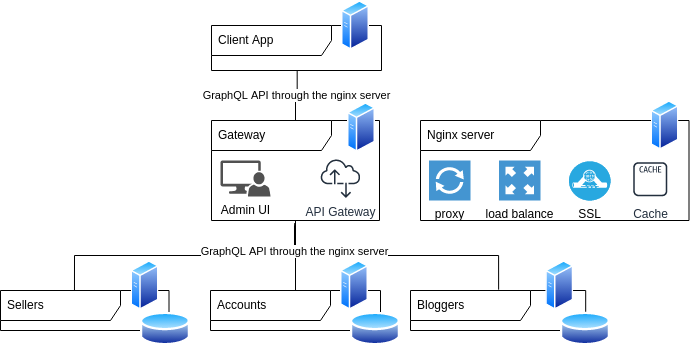
\includegraphics[width=\textwidth]{srs}
		\caption{Thiết kế chung của hệ thống}
	\end{center}
\end{figure}
Hệ thống thiết kế hướng dịch vụ chia làm 3 dịch vụ nhỏ là: sellers, accounts và bloggers. Tại máy chủ gateway có nhiệm vụ phân tích truy vấn đồ thị thành nhiều đồ thị con và gửi đến các dịch vụ sử lí. Sau đó gộp kết quả lại và trả về cho truy vấn. Gateway đồng thời cũng cũng cấp giao diện quản lí chung cho tất cả các dịch vụ.
\subsection{Sơ đồ ca sử dụng}
% https://www.uml-diagrams.org/use-case-diagrams.html

\begin{figure}[h!]
	\centering
	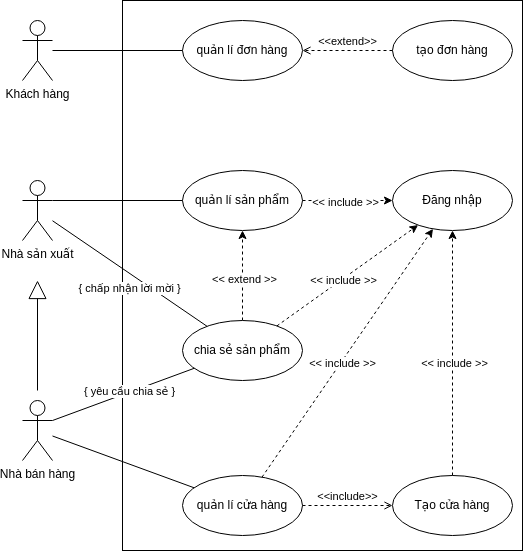
\includegraphics[width=0.6\textwidth]{usecase-usecase}
	\caption{Sơ đồ ca sử dụng tổng quát}
\end{figure}

\begin{figure}[h!]
	\begin{center}	
		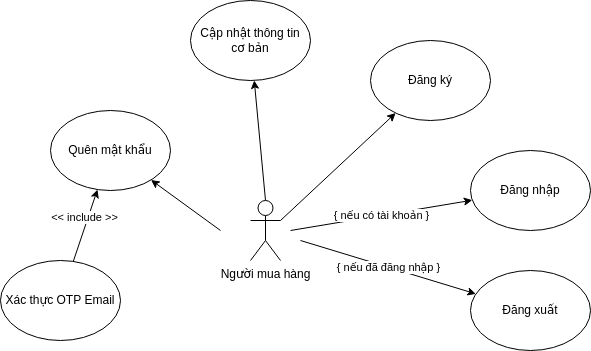
\includegraphics[width=0.6\textwidth]{usecase-user-login}
		\caption{Sơ đồ ca đăng nhập}
	\end{center}
\end{figure}


\begin{figure}[h!]
	\begin{center}	
		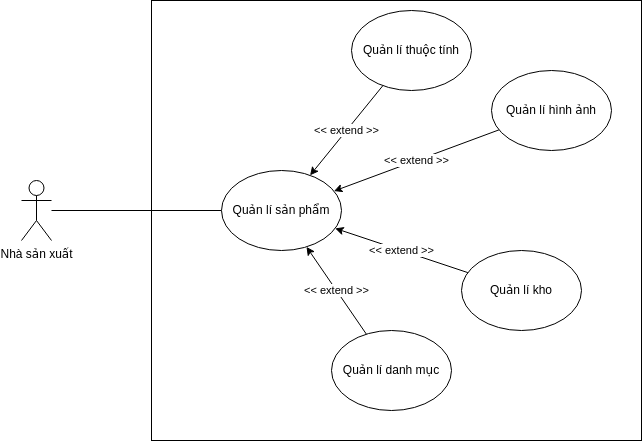
\includegraphics[width=0.6\textwidth]{usecase-sellers}
		\caption{Sơ đồ ca quản lí sản phẩm}
	\end{center}
\end{figure}


\begin{figure}[h!]
	\begin{center}	
		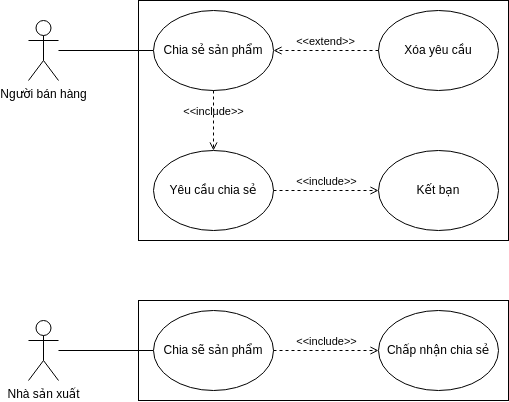
\includegraphics[width=0.6\textwidth]{usecase-contract}
		\caption{Sơ đồ ca yêu cầu chia sẻ}
	\end{center}
\end{figure}


\begin{figure}[h!]
	\begin{center}	
		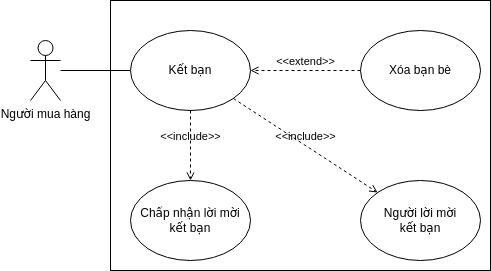
\includegraphics[width=0.6\textwidth]{usecase-relationship}
		\caption{Sơ đồ ca trường hợp kết bạn}
	\end{center}
\end{figure}



\begin{figure}[h!]
	\begin{center}	
		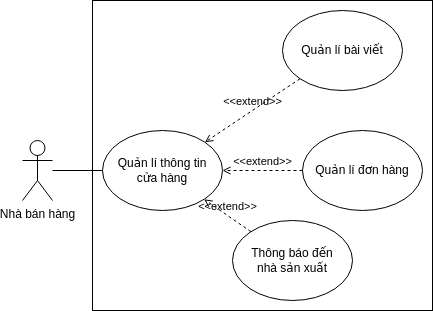
\includegraphics[width=0.5\textwidth]{usecase-store}
		\caption{Sơ đồ ca trường hợp quản lí cửa hàng}
	\end{center}
\end{figure}

\begin{figure}[h!]
	\begin{center}	
		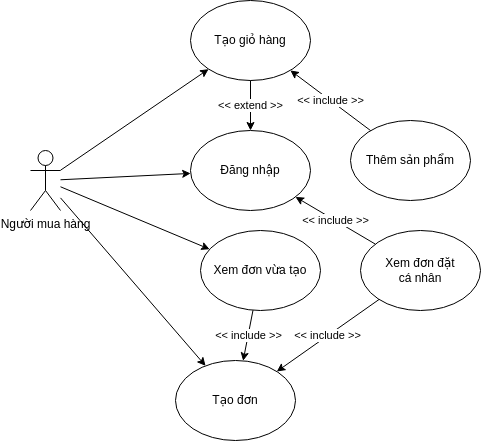
\includegraphics[width=0.6\textwidth]{usecase-order}
		\caption{Sơ đồ ca đặt hàng}
	\end{center}
\end{figure}

% Tính năng chia sẻ là khi lời mời được chấp nhận, sản phẩm của trang thương mại điện tử này có thể hiển thị và đặt mua ở trên trang khác. Nếu có cập nhật thì sản phẩm sẽ tự động đồng bộ.

\begin{figure}[h!]
	\begin{center}	
		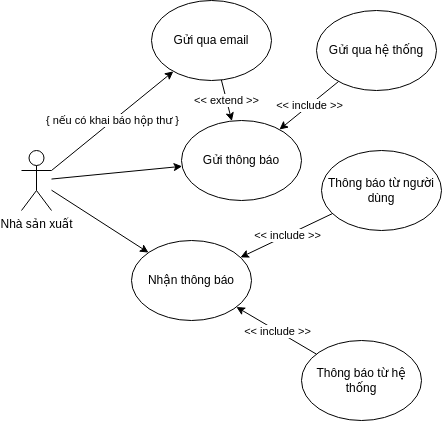
\includegraphics[width=0.5\textwidth]{usecase-notification}
		\caption{Sơ đồ ca trường hợp thông báo}
	\end{center}
\end{figure}
\subsection{Sơ đồ hoạt động}
% https://www.uml-diagrams.org/activity-diagrams.html

\begin{figure}[h!]
	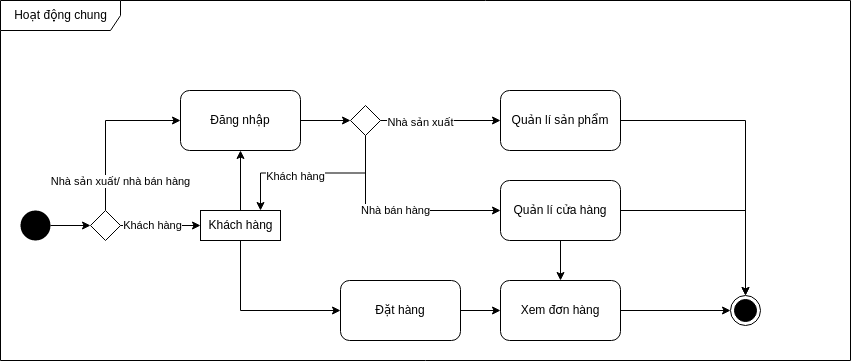
\includegraphics[width=\textwidth]{activity}
	\caption{Sơ đồ hoạt động tổng quát}
\end{figure}


\begin{figure}[h!]
	\begin{center}	
		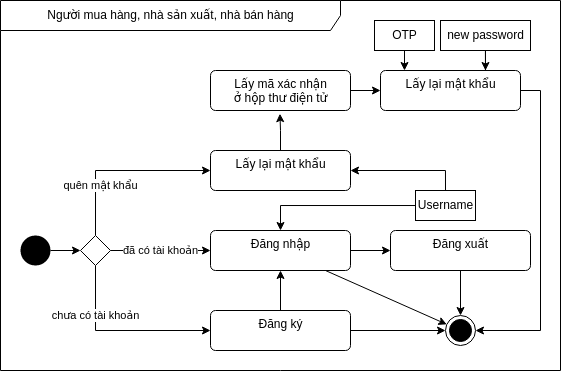
\includegraphics[width=0.8\textwidth]{activity-login}
		\caption{Sơ đồ hoạt động đăng nhập}
	\end{center}
\end{figure}


\begin{figure}[h!]
	\begin{center}	
		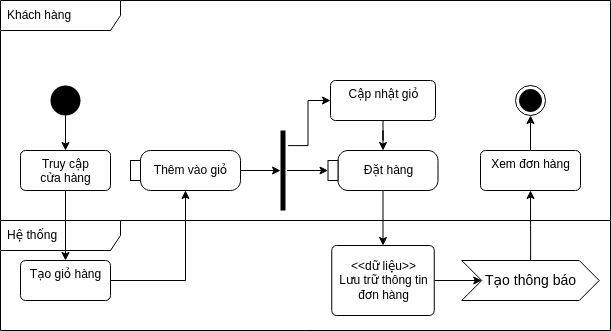
\includegraphics[width=0.8\textwidth]{activity-order}
		\caption{Sơ đồ hoạt động đặt hàng}
	\end{center}
\end{figure}
\begin{figure}[h!]
	\begin{center}	
		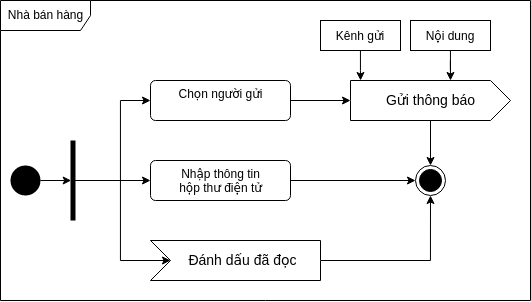
\includegraphics[width=0.8\textwidth]{activity-notification}
		\caption{Sơ đồ hoạt động thông báo}
	\end{center}
\end{figure}



\begin{figure}[h!]
	\begin{center}	
		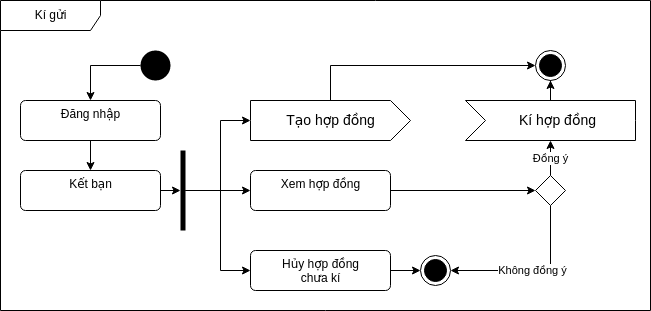
\includegraphics[width=0.8\textwidth]{activity-contract}
		\caption{Sơ đồ hoạt động yêu cầu chia sẻ}
	\end{center}
\end{figure}

\begin{figure}[h!]
	\begin{center}	
		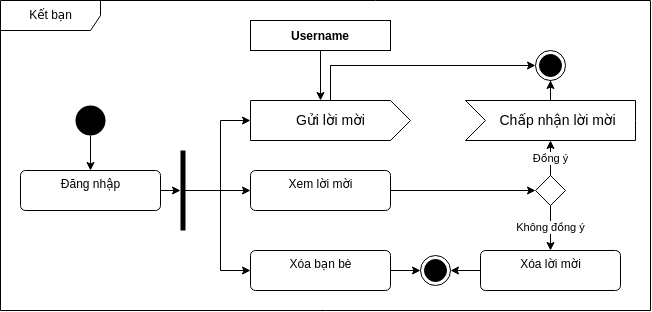
\includegraphics[width=0.8\textwidth]{activity-relationship}
		\caption{Sơ đồ hoạt động kết bạn}
	\end{center}
\end{figure}

%\begin{figure}[h!]
%	\begin{center}	
%		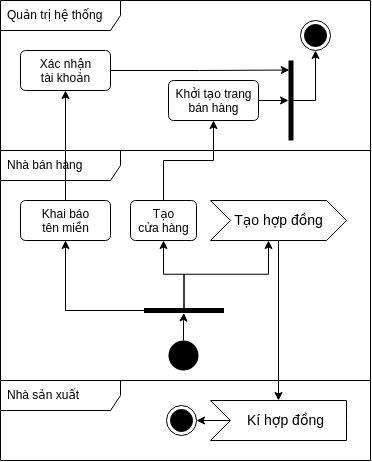
\includegraphics[width=0.6\textwidth]{activity-store}
%		\caption{Sơ đồ hoạt động quản lí cửa hàng}
%	\end{center}
%\end{figure}
\subsection{Sơ đồ tuần tự}
% https://www.uml-diagrams.org/sequence-diagrams.html


\begin{figure}[h!]
	\begin{center}	
		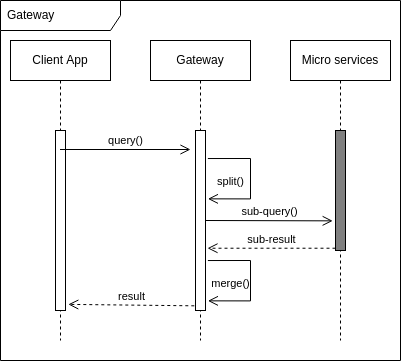
\includegraphics[width=0.6\textwidth]{sequence-gateway}
		\caption{Sơ đồ tuần tự hoạt động của gateway}
	\end{center}
\end{figure}


\begin{figure}[h!]
	\begin{center}	
		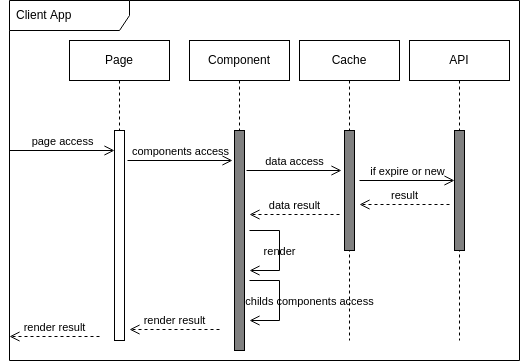
\includegraphics[width=0.6\textwidth]{sequence-component}
		\caption{Sơ đồ tuần tự kết xuất giao diện}
	\end{center}
\end{figure}

\begin{figure}[h!]
	\begin{center}	
		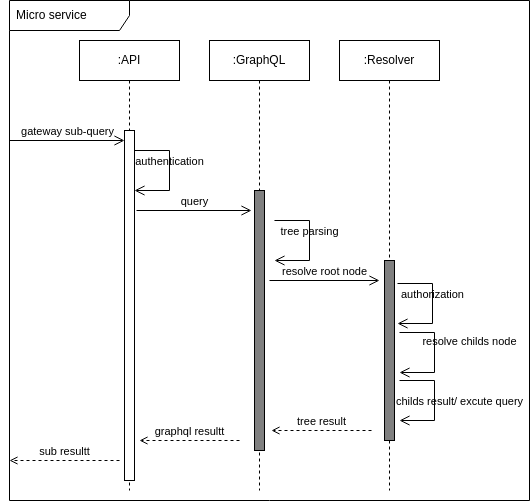
\includegraphics[width=0.6\textwidth]{sequence-service}
		\caption{Sơ đồ tuần tự xử lí truy vấns}
	\end{center}
\end{figure}


% \section{Thiết kế cấu trúc}\label{section:design}
%\subsection{Sơ đồ lớp}
% % https://www.uml-diagrams.org/package-diagrams-overview.html
\subsection{Sơ đồ đóng gói}
% https://www.uml-diagrams.org/component-diagrams.html
\subsection{Sơ đồ thành phần}

\begin{figure}[h!]
	\begin{center}	
		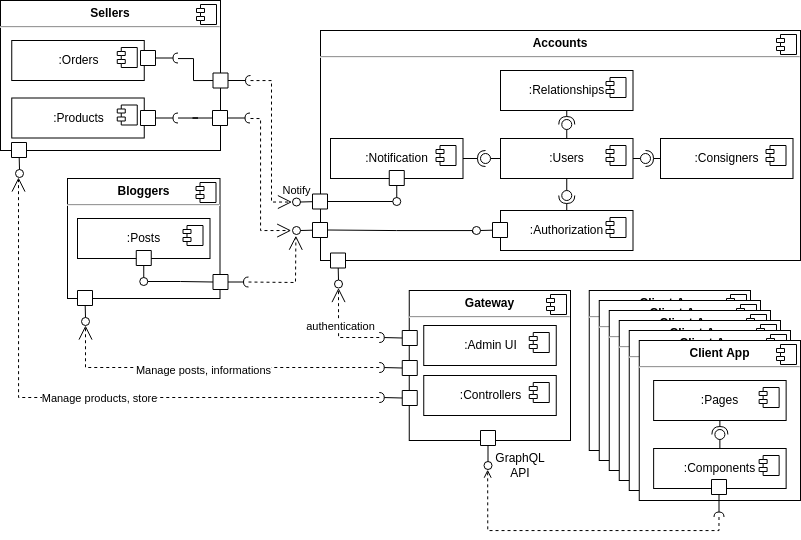
\includegraphics[width=\textwidth]{component}
		\caption{Sơ đồ thành phần hệ thống}
	\end{center}
\end{figure}
% https://www.uml-diagrams.org/deployment-diagrams-overview.html
\subsection{Sơ đồ phát hành}
\begin{figure}[h!]
	\begin{center}	
		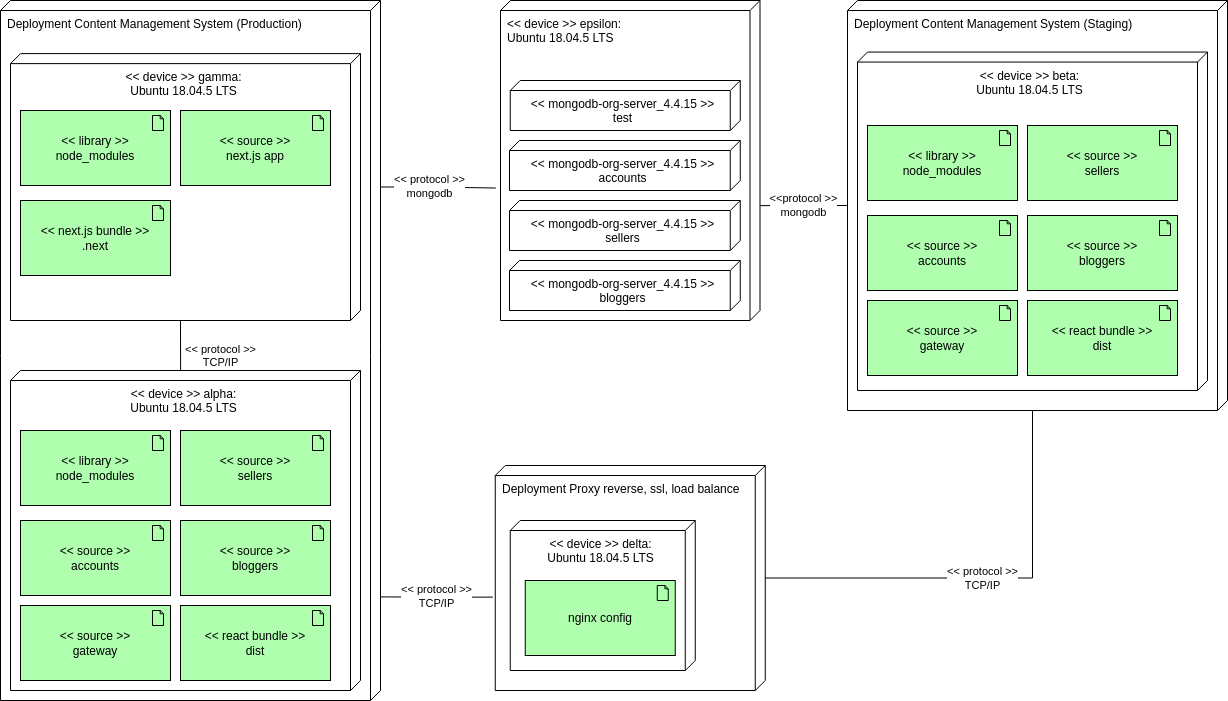
\includegraphics[width=\textwidth]{deployment}
		\caption{Sơ đồ phát hành tổng quát}
	\end{center}
\end{figure}

\subsection{Dữ liệu}
\begin{table}[h!]
\begin{center}
\begin{tabular}{ |l|l|l| } 
	\hline
	Tên & Kiểu & Mô tả \\
	\hline
	to & Virtual & \dotfill \\
isAccepted & Checkbox & \dotfill \\
key & Text & \dotfill \\ 
	\hline
\end{tabular}
	\caption{Mô tả bảng ContractConsignment.}
	\label{table:ContractConsignment}
\end{center}
\end{table}


\begin{table}[h!]
\begin{center}
\begin{tabular}{ |l|l|l| } 
	\hline
	Tên & Kiểu & Mô tả \\
	\hline
	content & Markdown & \dotfill \\
status & Select & \dotfill \\
price & Virtual & \dotfill \\ 
	\hline
\end{tabular}
	\caption{Mô tả bảng ContractLabor.}
	\label{table:ContractLabor}
\end{center}
\end{table}


\begin{table}[h!]
\begin{center}
\begin{tabular}{ |l|l|l| } 
	\hline
	Tên & Kiểu & Mô tả \\
	\hline
	content & Text & \dotfill \\ 
	\hline
\end{tabular}
	\caption{Mô tả bảng InteractionComment.}
	\label{table:InteractionComment}
\end{center}
\end{table}


\begin{table}[h!]
\begin{center}
\begin{tabular}{ |l|l|l| } 
	\hline
	Tên & Kiểu & Mô tả \\
	\hline
	emoji & Select & \dotfill \\ 
	\hline
\end{tabular}
	\caption{Mô tả bảng InteractionReaction.}
	\label{table:InteractionReaction}
\end{center}
\end{table}


\begin{table}[h!]
\begin{center}
\begin{tabular}{ |l|l|l| } 
	\hline
	Tên & Kiểu & Mô tả \\
	\hline
	status & Checkbox & \dotfill \\
item & MongoId & \dotfill \\ 
	\hline
\end{tabular}
	\caption{Mô tả bảng Interaction.}
	\label{table:Interaction}
\end{center}
\end{table}


\begin{table}[h!]
\begin{center}
\begin{tabular}{ |l|l|l| } 
	\hline
	Tên & Kiểu & Mô tả \\
	\hline
	username & Text & \dotfill \\
password & Text & \dotfill \\
host & Text & \dotfill \\
port & Integer & \dotfill \\
secure & Checkbox & \dotfill \\
name & Text & \dotfill \\ 
	\hline
\end{tabular}
	\caption{Mô tả bảng NotificationMailer.}
	\label{table:NotificationMailer}
\end{center}
\end{table}


\begin{table}[h!]
\begin{center}
\begin{tabular}{ |l|l|l| } 
	\hline
	Tên & Kiểu & Mô tả \\
	\hline
	chanel & Select & \dotfill \\
subject & Text & \dotfill \\
text & Text & \dotfill \\
seen & Checkbox & \dotfill \\ 
	\hline
\end{tabular}
	\caption{Mô tả bảng Notification.}
	\label{table:Notification}
\end{center}
\end{table}


\begin{table}[h!]
\begin{center}
\begin{tabular}{ |l|l|l| } 
	\hline
	Tên & Kiểu & Mô tả \\
	\hline
	username & Text & \dotfill \\
to & Virtual & \dotfill \\
isAccepted & Checkbox & \dotfill \\
key & Text & \dotfill \\
consignment & Virtual & \dotfill \\ 
	\hline
\end{tabular}
	\caption{Mô tả bảng Relationship.}
	\label{table:Relationship}
\end{center}
\end{table}


\begin{table}[h!]
\begin{center}
\begin{tabular}{ |l|l|l| } 
	\hline
	Tên & Kiểu & Mô tả \\
	\hline
	isAccepted & Checkbox & \dotfill \\
key & Text & \dotfill \\ 
	\hline
\end{tabular}
	\caption{Mô tả bảng TeamInvitation.}
	\label{table:TeamInvitation}
\end{center}
\end{table}


\begin{table}[h!]
\begin{center}
\begin{tabular}{ |l|l|l| } 
	\hline
	Tên & Kiểu & Mô tả \\
	\hline
	name & Text & \dotfill \\
description & Text & \dotfill \\ 
	\hline
\end{tabular}
	\caption{Mô tả bảng Team.}
	\label{table:Team}
\end{center}
\end{table}


\begin{table}[h!]
\begin{center}
\begin{tabular}{ |l|l|l| } 
	\hline
	Tên & Kiểu & Mô tả \\
	\hline
	username & Text & \dotfill \\
password & Password & \dotfill \\
phone & Text & \dotfill \\
email & Text & \dotfill \\
name & Text & \dotfill \\
fullname & Text & \dotfill \\
avatar & File & \dotfill \\
abount & Text & \dotfill \\
domain & Text & \dotfill \\
isAdmin & Checkbox & \dotfill \\
isSeller & Checkbox & \dotfill \\
isActive & Checkbox & \dotfill \\
forgotAt & DateTime & \dotfill \\ 
	\hline
\end{tabular}
	\caption{Mô tả bảng User.}
	\label{table:User}
\end{center}
\end{table}


\begin{table}[h!]
\begin{center}
\begin{tabular}{ |l|l|l| } 
	\hline
	Tên & Kiểu & Mô tả \\
	\hline
	listKey & Text & \dotfill \\
count & Integer & \dotfill \\
of & MongoId & \dotfill \\ 
	\hline
\end{tabular}
	\caption{Mô tả bảng View.}
	\label{table:View}
\end{center}
\end{table}


\begin{table}[h!]
\begin{center}
\begin{tabular}{ |l|l|l| } 
	\hline
	Tên & Kiểu & Mô tả \\
	\hline
	price & Currency & \dotfill \\ 
	\hline
\end{tabular}
	\caption{Mô tả bảng WorkPaid.}
	\label{table:WorkPaid}
\end{center}
\end{table}


\begin{table}[h!]
\begin{center}
\begin{tabular}{ |l|l|l| } 
	\hline
	Tên & Kiểu & Mô tả \\
	\hline
	title & Text & \dotfill \\
price & Currency & \dotfill \\
unit & Select & \dotfill \\ 
	\hline
\end{tabular}
	\caption{Mô tả bảng WorkType.}
	\label{table:WorkType}
\end{center}
\end{table}


\begin{table}[h!]
\begin{center}
\begin{tabular}{ |l|l|l| } 
	\hline
	Tên & Kiểu & Mô tả \\
	\hline
	amount & Integer & \dotfill \\
content & Text & \dotfill \\
confirmAt & CalendarDay & \dotfill \\ 
	\hline
\end{tabular}
	\caption{Mô tả bảng Work.}
	\label{table:Work}
\end{center}
\end{table}


\begin{table}[h!]
\begin{center}
\begin{tabular}{ |l|l|l| } 
	\hline
	Tên & Kiểu & Mô tả \\
	\hline
	name & Text & \dotfill \\
slogan & Text & \dotfill \\
image & File & \dotfill \\
description & Text & \dotfill \\
url & Text & \dotfill \\
type & Select & \dotfill \\
size & Virtual & \dotfill \\ 
	\hline
\end{tabular}
	\caption{Mô tả bảng Banner.}
	\label{table:Banner}
\end{center}
\end{table}


\begin{table}[h!]
\begin{center}
\begin{tabular}{ |l|l|l| } 
	\hline
	Tên & Kiểu & Mô tả \\
	\hline
	phone & Text & \dotfill \\
name & Text & \dotfill \\
address & Text & \dotfill \\
email & Text & \dotfill \\
note & Text & \dotfill \\
message & Text & \dotfill \\
isDefault & Checkbox & \dotfill \\ 
	\hline
\end{tabular}
	\caption{Mô tả bảng Contact.}
	\label{table:Contact}
\end{center}
\end{table}


\begin{table}[h!]
\begin{center}
\begin{tabular}{ |l|l|l| } 
	\hline
	Tên & Kiểu & Mô tả \\
	\hline
	store & Text & \dotfill \\
logo & File & \dotfill \\
slogan & Text & \dotfill \\
address & Text & \dotfill \\
phone & Text & \dotfill \\
email & Text & \dotfill \\
intro & Editor & \dotfill \\
contact & Editor & \dotfill \\
twitter & Text & \dotfill \\
instagram & Text & \dotfill \\
pinterest & Text & \dotfill \\
youtube & Text & \dotfill \\
googlePlus & Text & \dotfill \\
googleMap & Text & \dotfill \\
zalo & Text & \dotfill \\
greeting & Text & \dotfill \\
pageId & Text & \dotfill \\
pixelId & Text & \dotfill \\
gtag & Text & \dotfill \\
shipMoneySupport & Integer & \dotfill \\
ship & Editor & \dotfill \\
transfer & Editor & \dotfill \\
color & Color & \dotfill \\
colorMode & Select & \dotfill \\
ordering & Checkbox & \dotfill \\
moit & Text & \dotfill \\
mst & Text & \dotfill \\
language & Select & \dotfill \\
translations & Translate & \dotfill \\ 
	\hline
\end{tabular}
	\caption{Mô tả bảng Page.}
	\label{table:Page}
\end{center}
\end{table}


\begin{table}[h!]
\begin{center}
\begin{tabular}{ |l|l|l| } 
	\hline
	Tên & Kiểu & Mô tả \\
	\hline
	value & Text & \dotfill \\
file & File & \dotfill \\ 
	\hline
\end{tabular}
	\caption{Mô tả bảng ProductAttributeValue.}
	\label{table:ProductAttributeValue}
\end{center}
\end{table}


\begin{table}[h!]
\begin{center}
\begin{tabular}{ |l|l|l| } 
	\hline
	Tên & Kiểu & Mô tả \\
	\hline
	label & Text & \dotfill \\
name & Text & \dotfill \\
language & Select & \dotfill \\
translations & Translate & \dotfill \\ 
	\hline
\end{tabular}
	\caption{Mô tả bảng ProductAttribute.}
	\label{table:ProductAttribute}
\end{center}
\end{table}


\begin{table}[h!]
\begin{center}
\begin{tabular}{ |l|l|l| } 
	\hline
	Tên & Kiểu & Mô tả \\
	\hline
	name & Text & \dotfill \\
url & Slug & \dotfill \\
language & Select & \dotfill \\
translations & Translate & \dotfill \\ 
	\hline
\end{tabular}
	\caption{Mô tả bảng ProductBrand.}
	\label{table:ProductBrand}
\end{center}
\end{table}


\begin{table}[h!]
\begin{center}
\begin{tabular}{ |l|l|l| } 
	\hline
	Tên & Kiểu & Mô tả \\
	\hline
	sale & Integer & \dotfill \\
price & Integer & \dotfill \\
percent & Virtual & \dotfill \\
isInCart & Virtual & \dotfill \\
quantity & Integer & \dotfill \\ 
	\hline
\end{tabular}
	\caption{Mô tả bảng ProductCartItem.}
	\label{table:ProductCartItem}
\end{center}
\end{table}


\begin{table}[h!]
\begin{center}
\begin{tabular}{ |l|l|l| } 
	\hline
	Tên & Kiểu & Mô tả \\
	\hline
	 
	\hline
\end{tabular}
	\caption{Mô tả bảng ProductCart.}
	\label{table:ProductCart}
\end{center}
\end{table}


\begin{table}[h!]
\begin{center}
\begin{tabular}{ |l|l|l| } 
	\hline
	Tên & Kiểu & Mô tả \\
	\hline
	name & Text & \dotfill \\
description & Editor & \dotfill \\
file & File & \dotfill \\
prioritize & Integer & \dotfill \\
url & Slug & \dotfill \\
root & Checkbox & \dotfill \\
language & Select & \dotfill \\
translations & Translate & \dotfill \\ 
	\hline
\end{tabular}
	\caption{Mô tả bảng ProductCategory.}
	\label{table:ProductCategory}
\end{center}
\end{table}


\begin{table}[h!]
\begin{center}
\begin{tabular}{ |l|l|l| } 
	\hline
	Tên & Kiểu & Mô tả \\
	\hline
	code & Text & \dotfill \\
type & Select & \dotfill \\
value & Integer & \dotfill \\
name & Text & \dotfill \\
description & Text & \dotfill \\
condition & Integer & \dotfill \\
image & File & \dotfill \\
url & Slug & \dotfill \\
language & Select & \dotfill \\
translations & Translate & \dotfill \\ 
	\hline
\end{tabular}
	\caption{Mô tả bảng ProductDiscount.}
	\label{table:ProductDiscount}
\end{center}
\end{table}


\begin{table}[h!]
\begin{center}
\begin{tabular}{ |l|l|l| } 
	\hline
	Tên & Kiểu & Mô tả \\
	\hline
	name & Text & \dotfill \\
url & Slug & \dotfill \\
language & Select & \dotfill \\
translations & Translate & \dotfill \\ 
	\hline
\end{tabular}
	\caption{Mô tả bảng ProductHashtag.}
	\label{table:ProductHashtag}
\end{center}
\end{table}


\begin{table}[h!]
\begin{center}
\begin{tabular}{ |l|l|l| } 
	\hline
	Tên & Kiểu & Mô tả \\
	\hline
	value & Text & \dotfill \\
color & Select & \dotfill \\ 
	\hline
\end{tabular}
	\caption{Mô tả bảng ProductOrderStatus.}
	\label{table:ProductOrderStatus}
\end{center}
\end{table}


\begin{table}[h!]
\begin{center}
\begin{tabular}{ |l|l|l| } 
	\hline
	Tên & Kiểu & Mô tả \\
	\hline
	code & Text & \dotfill \\
isExport & Checkbox & \dotfill \\
payment & Select & \dotfill \\
saving & Integer & \dotfill \\
total & Integer & \dotfill \\
notification & MongoId & \dotfill \\ 
	\hline
\end{tabular}
	\caption{Mô tả bảng ProductOrder.}
	\label{table:ProductOrder}
\end{center}
\end{table}


\begin{table}[h!]
\begin{center}
\begin{tabular}{ |l|l|l| } 
	\hline
	Tên & Kiểu & Mô tả \\
	\hline
	quantity & Integer & \dotfill \\
image & File & \dotfill \\ 
	\hline
\end{tabular}
	\caption{Mô tả bảng ProductStock.}
	\label{table:ProductStock}
\end{center}
\end{table}


\begin{table}[h!]
\begin{center}
\begin{tabular}{ |l|l|l| } 
	\hline
	Tên & Kiểu & Mô tả \\
	\hline
	image & File & \dotfill \\
images & Images & \dotfill \\
name & Text & \dotfill \\
price & Currency & \dotfill \\
sale & Currency & \dotfill \\
percent & Virtual & \dotfill \\
status & Select & \dotfill \\
description & Editor & \dotfill \\
detail & File & \dotfill \\
guide & Editor & \dotfill \\
isDraft & Checkbox & \dotfill \\
isOutOfStock & Checkbox & \dotfill \\
sku & Text & \dotfill \\
gs1 & Text & \dotfill \\
url & Slug & \dotfill \\
sold & Virtual & \dotfill \\
language & Select & \dotfill \\
translations & Translate & \dotfill \\ 
	\hline
\end{tabular}
	\caption{Mô tả bảng Product.}
	\label{table:Product}
\end{center}
\end{table}


\begin{table}[h!]
\begin{center}
\begin{tabular}{ |l|l|l| } 
	\hline
	Tên & Kiểu & Mô tả \\
	\hline
	item & MongoId & \dotfill \\
listKey & Text & \dotfill \\
fieldName & Text & \dotfill \\
lang & Text & \dotfill \\
content & Text & \dotfill \\ 
	\hline
\end{tabular}
	\caption{Mô tả bảng Translate.}
	\label{table:Translate}
\end{center}
\end{table}


\begin{table}[h!]
\begin{center}
\begin{tabular}{ |l|l|l| } 
	\hline
	Tên & Kiểu & Mô tả \\
	\hline
	file & File & \dotfill \\
address & Text & \dotfill \\ 
	\hline
\end{tabular}
	\caption{Mô tả bảng UploadFile.}
	\label{table:UploadFile}
\end{center}
\end{table}


\begin{table}[h!]
\begin{center}
\begin{tabular}{ |l|l|l| } 
	\hline
	Tên & Kiểu & Mô tả \\
	\hline
	file & File & \dotfill \\
alt & Text & \dotfill \\ 
	\hline
\end{tabular}
	\caption{Mô tả bảng UploadImage.}
	\label{table:UploadImage}
\end{center}
\end{table}


\begin{table}[h!]
\begin{center}
\begin{tabular}{ |l|l|l| } 
	\hline
	Tên & Kiểu & Mô tả \\
	\hline
	title & Text & \dotfill \\
body & Markdown & \dotfill \\
prioritize & Integer & \dotfill \\ 
	\hline
\end{tabular}
	\caption{Mô tả bảng FAQ.}
	\label{table:FAQ}
\end{center}
\end{table}


\begin{table}[h!]
\begin{center}
\begin{tabular}{ |l|l|l| } 
	\hline
	Tên & Kiểu & Mô tả \\
	\hline
	name & Text & \dotfill \\
image & File & \dotfill \\
description & Markdown & \dotfill \\
content & Markdown & \dotfill \\ 
	\hline
\end{tabular}
	\caption{Mô tả bảng Feature.}
	\label{table:Feature}
\end{center}
\end{table}


\begin{table}[h!]
\begin{center}
\begin{tabular}{ |l|l|l| } 
	\hline
	Tên & Kiểu & Mô tả \\
	\hline
	name & Text & \dotfill \\
image & File & \dotfill \\
root & Checkbox & \dotfill \\
description & Markdown & \dotfill \\
prioritize & Integer & \dotfill \\
color & Color & \dotfill \\
url & Slug & \dotfill \\ 
	\hline
\end{tabular}
	\caption{Mô tả bảng PostHashtag.}
	\label{table:PostHashtag}
\end{center}
\end{table}


\begin{table}[h!]
\begin{center}
\begin{tabular}{ |l|l|l| } 
	\hline
	Tên & Kiểu & Mô tả \\
	\hline
	title & Text & \dotfill \\
thumbnail & File & \dotfill \\
content & Markdown & \dotfill \\
prioritize & Integer & \dotfill \\
embed & Text & \dotfill \\
description & Text & \dotfill \\
keywords & Text & \dotfill \\
url & Slug & \dotfill \\
body & Text & \dotfill \\ 
	\hline
\end{tabular}
	\caption{Mô tả bảng Post.}
	\label{table:Post}
\end{center}
\end{table}


\begin{table}[h!]
\begin{center}
\begin{tabular}{ |l|l|l| } 
	\hline
	Tên & Kiểu & Mô tả \\
	\hline
	name & Text & \dotfill \\
image & File & \dotfill \\
description & Text & \dotfill \\
content & Markdown & \dotfill \\ 
	\hline
\end{tabular}
	\caption{Mô tả bảng Service.}
	\label{table:Service}
\end{center}
\end{table}


\begin{table}[h!]
\begin{center}
\begin{tabular}{ |l|l|l| } 
	\hline
	Tên & Kiểu & Mô tả \\
	\hline
	name & Text & \dotfill \\
profile & Text & \dotfill \\
description & Text & \dotfill \\
image & File & \dotfill \\ 
	\hline
\end{tabular}
	\caption{Mô tả bảng Testimonial.}
	\label{table:Testimonial}
\end{center}
\end{table}


\fontsize{13px}{13px}\selectfont\justifying

\chapter{TRIỂN KHAI VÀ ĐÁNH GIÁ}\label{section:dev}

\section{Triển khai}

\subsection{Cấu hình máy chủ}

\begin{itemize}
	\item \textbf{Máy chủ \gls{staging}} Virtual CPUs: 1. Memory (RAM): 2048 MB. Disk: 15 GB
	
	\item \textbf{Máy chủ \gls{production}}. Virtual CPUs: 1. Memory (RAM): 1536 MB. Disk: 15 GB
	
	\item \textbf{Máy chủ database}. Virtual CPUs: 1. Memory (RAM): 1536 MB. Disk: 15 GB
	
	\item \textbf{Máy chủ proxy}. Virtual CPUs: 1. Memory (RAM): 1536 MB. Disk: 15 GB
\end{itemize}
\subsection{Cài đặt tiến trình}


\subsubsection{Máy chủ \gls{staging}}
\begin{itemize}
	\item Tiến trình accounts chạy ở chế độ \gls{staging} kết nối với database test
	\item Tiến trình sellers chạy ở chế độ \gls{staging} kết nối với database test
	\item Tiến trình bloggers chạy ở chế độ \gls{staging} kết nối với database test
	\item Tiến trình gateway chạy ở chế độ \gls{staging} cung cấp giao diện quản lí mà sanbox để kiểm tra API.
\end{itemize}
\subsubsection{Máy chủ \gls{production}}
\begin{itemize}
	\item Tiến trình accounts chạy ở chế độ \emph{production} kết nối với database account
	\item Tiến trình  chạy ở chế độ \emph{production} kết nối với database seller
	\item Tiến trình bloggers chạy ở chế độ \emph{production} kết nối với database blogger
	\item Tiến trình gateway chạy ở chế độ \emph{production} cung cấp giao diện quản lí.
\end{itemize}

\subsubsection{Máy chủ database}
Cấu hình mongodb và cung cấp các database cho các môi trường phát hành.
\begin{itemize}
	\item account
	\item seller
	\item blogger
	\item test (cho môi trường \gls{staging})
\end{itemize}
\subsubsection{Máy chủ proxy}
Cấu hình liên kết tên miền với cổng tiến trình của các máy chủ trong hệ thống. Đăng ký chứng thực \acrshort{ssl}. Sử dụng các thuật toán cân bằng tải có sẵn để điều phối \gls{request}.

\subsection{Hình ảnh triển khai}
\FloatBarrier
\begin{figure}[!htbp]\fontsize{13px}{13px}\selectfont
\centering
		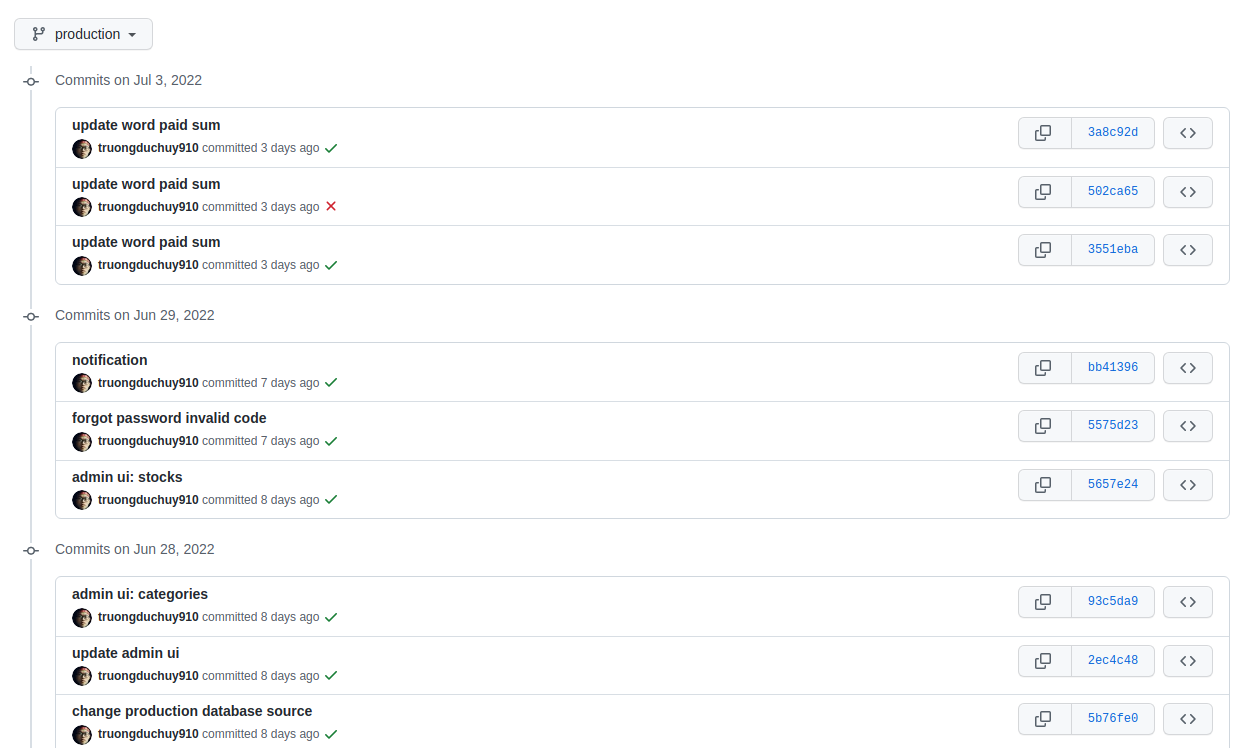
\includegraphics[width=\textwidth]{./results/commit}
		\caption{Lịch sử các phiên bản phát hành môi trường \gls{production}.}
\justifying
Các commit được triển khai thành công sẽ hiện dấu tích xanh. Khi có sự cố có thể quay về bản triển khai thành công trước đó. Là một phương án tốt khi có lỗ hổng trên môi trường \gls{production}.
	
\end{figure}
\clearpage
\FloatBarrier
\begin{figure}[!htbp]\fontsize{13px}{13px}\selectfont
\centering
		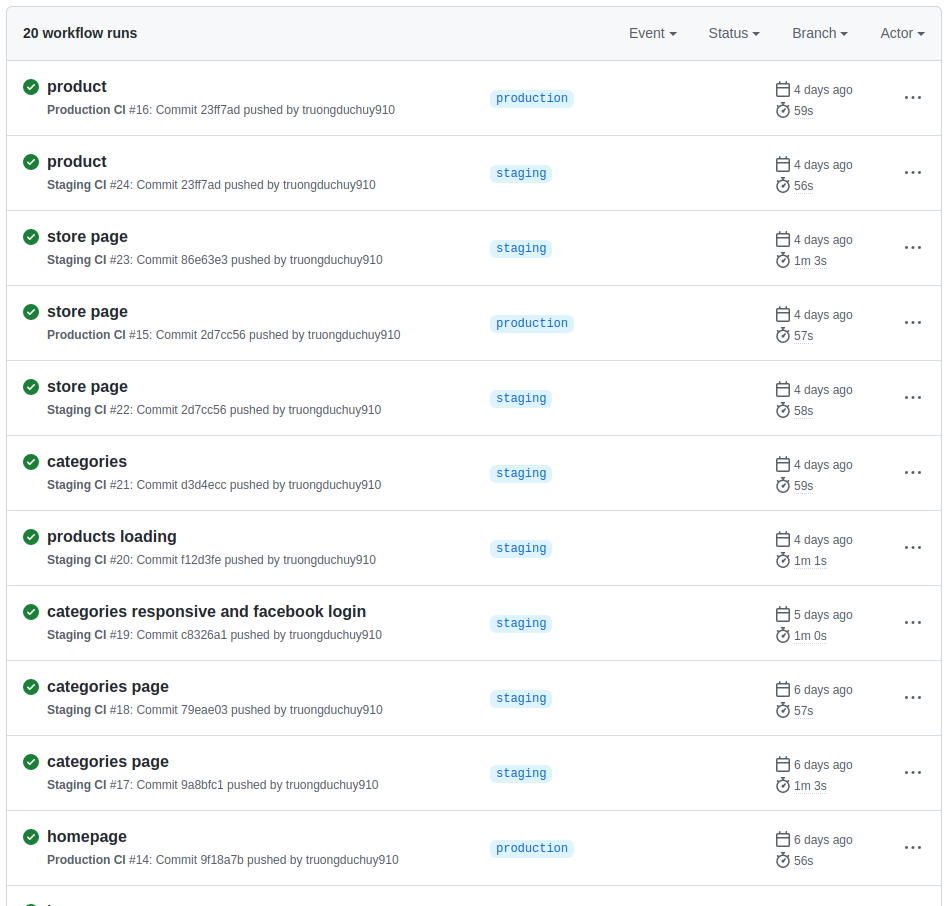
\includegraphics[width=\textwidth]{./results/deployments}
		\caption{Lịch sử cài đặt tiến trình ở các môi trường \gls{staging} và \gls{production} sử dụng CI/CD của github actions.}
\justifying
Lịch sử triển khai các commit trên các môi trường. Sau khi triển khai các tính năng trên môi trường \gls{staging} và trải qua công việc kiểm thử. Nếu không phát sinh vấn đề. Tất cả tính năng mới của \gls{staging} so với \gls{production} sẽ được triển khai bằng cách gộp mã nguồn của nhánh \gls{staging} vào nhánh \gls{production}.
	
\end{figure}
\clearpage
\begin{figure}[h!]\fontsize{13px}{13px}\selectfont
\centering
		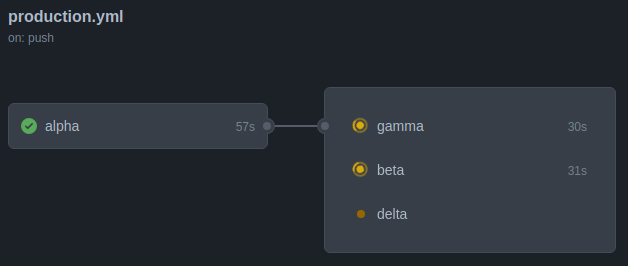
\includegraphics[width=\textwidth]{./results/jobs}
		\caption{Thông tin chi tiết khi sử dụng CI/CD chạy các bản sao của micro service trên nhiều máy chủ khác nhau}
\justifying
Hình trên mô tả máy chủ alpha là một máy chủ dự phòng của các máy chủ còn lại. Máy chủ alpha có khả năng dự phòng cho hầu hết các máy chủ dịch vụ khác. Nhưng ít khi được sử dụng. Khi việc triển diễn ra thành công trên máy chủ dự phòng, các máy chủ dịch vụ khác mới được triển khai để tránh trường hợp ảnh hưởng đến trải nghiệm phía người dùng.
\end{figure}


\begin{figure}[h!]\fontsize{13px}{13px}\selectfont
	\begin{center}	
		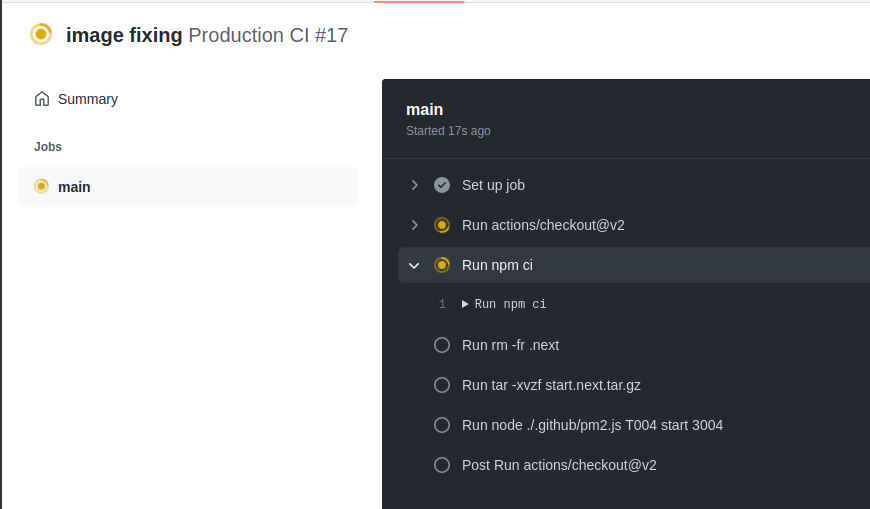
\includegraphics[width=\textwidth]{./results/production}
		\caption{Thông tin chi tiết các bước của một mirco-service sử dụng CI/CD}
	\end{center}
\end{figure}





\fontsize{13px}{13px}\selectfont\justifying

\subsection{Kết quả}
\subsubsection{Môi trường \Gls{staging}}
\FloatBarrier
\begin{figure}[!htbp]\fontsize{13px}{13px}\selectfont
\centering
		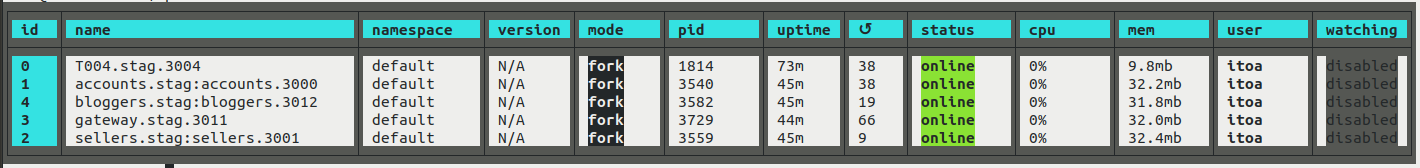
\includegraphics[width=\textwidth]{./results/vps-staging}
		\caption{Thông tin các tiến trình máy chủ \gls{staging}}
\justifying
Xem kết quả ứng dụng web tại fashion.ocopee.com
\end{figure}
\subsubsection{Môi trường \Gls{production}}
\FloatBarrier
\begin{figure}[!htbp]\fontsize{13px}{13px}\selectfont
\centering
		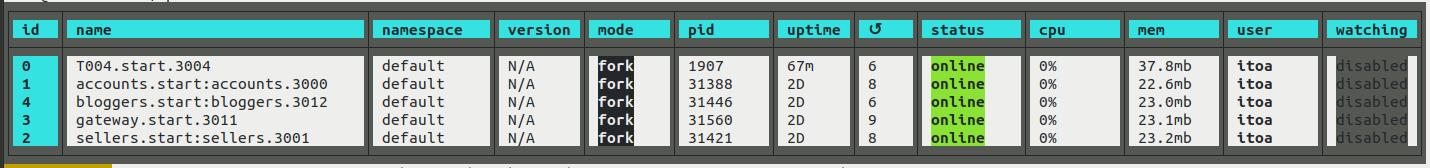
\includegraphics[width=\textwidth]{./results/vps-production}
		\caption{Thông tin các tiến trình máy chủ \gls{production}}
\justifying
Xem kết quả ứng dụng web tại ocopee.com
\end{figure}
\FloatBarrier
\begin{figure}[!htbp]\fontsize{13px}{13px}\selectfont
\centering
		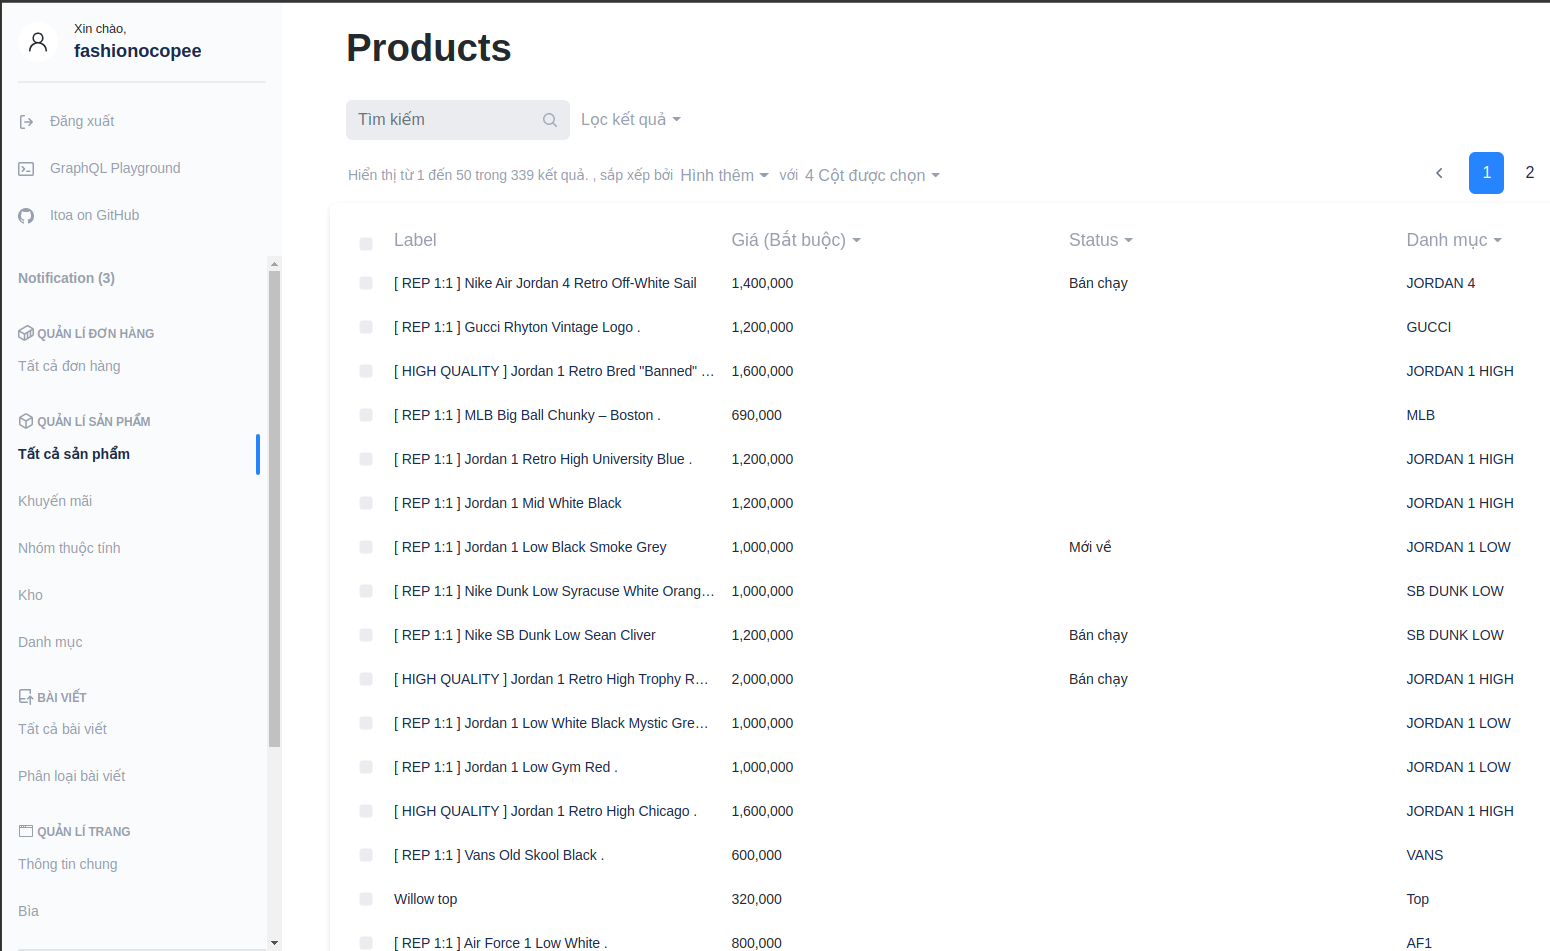
\includegraphics[width=\textwidth]{./results/product}
		\caption{Trang quản lí sản phẩm}
\justifying
\end{figure}
\clearpage
\subsubsection{Trang quản lí đơn hàng}
\FloatBarrier
\begin{figure}[!htbp]\fontsize{13px}{13px}\selectfont
\centering
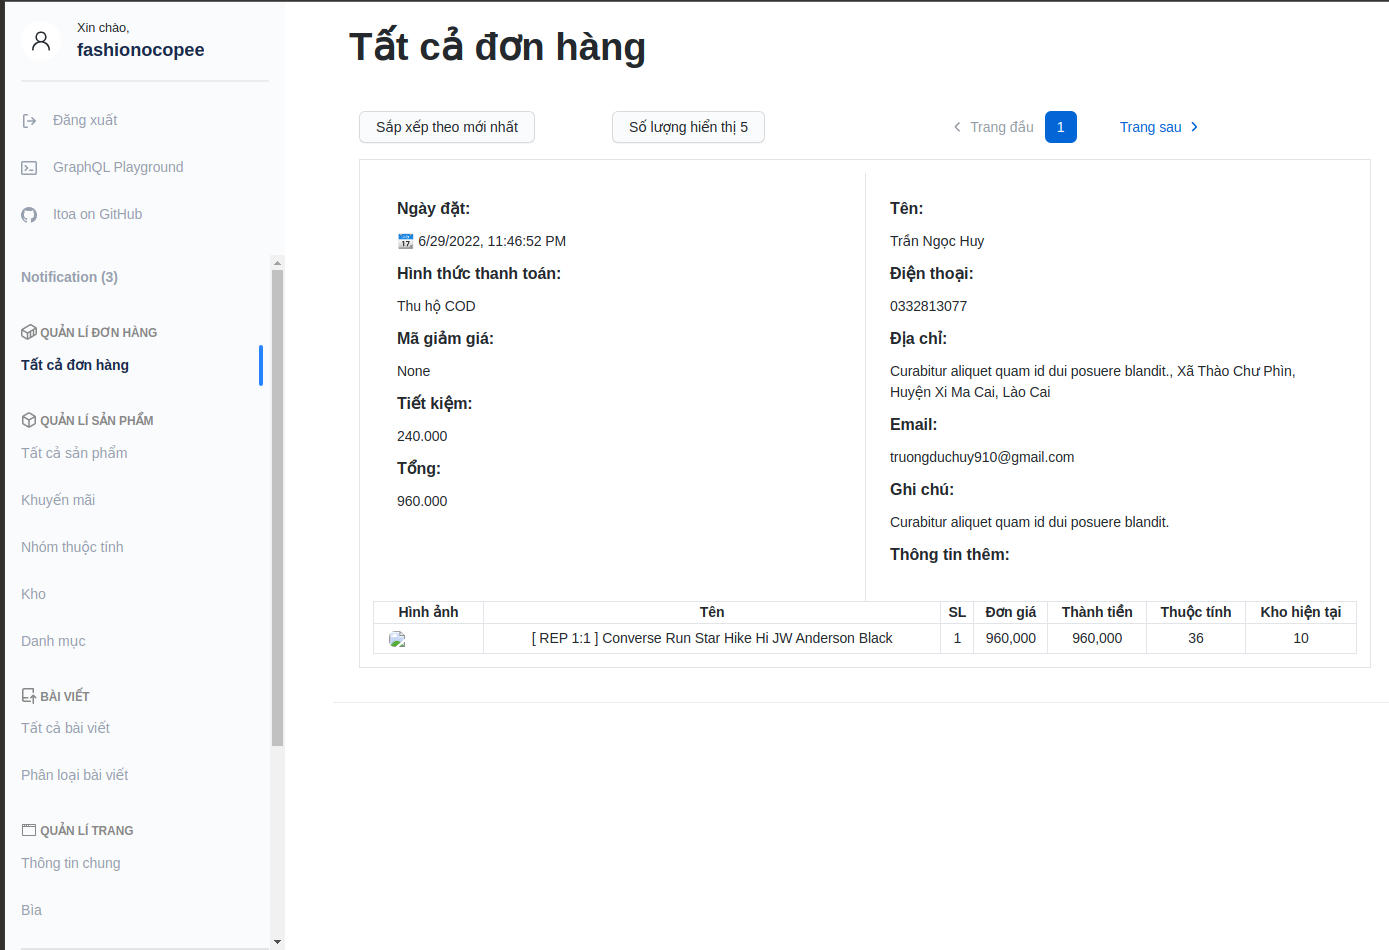
\includegraphics[width=\textwidth]{./results/order}
\caption{Trang quản lí đơn hàng}
\justifying
Trang quản lí thông tin đơn hàng dành cho nhà bán hàng cho phép nhà bán hàng xem thông tin người mua hàng để lại bao gồm: Địa chỉ nhận hàng, thông tin liên hệ, hình thức thanh toán, chi tiết đơn hàng và mã giảm giá đã sử dụng.
\end{figure}
\clearpage
\subsubsection{Trang kết bạn và chia sẻ sản phẩm}
\FloatBarrier
\begin{figure}[!htbp]\fontsize{13px}{13px}\selectfont
\centering
		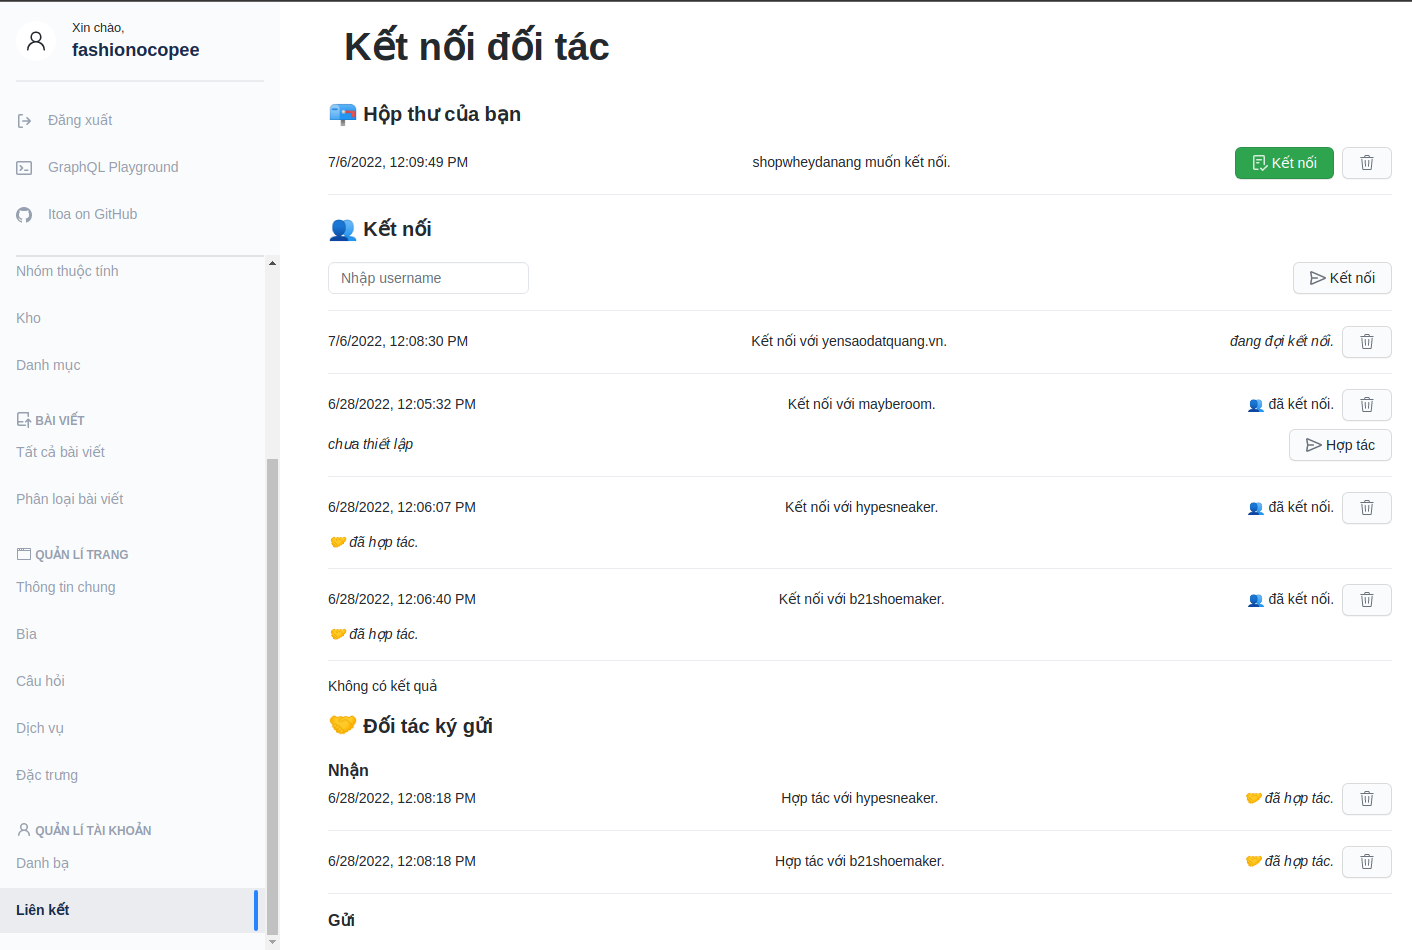
\includegraphics[width=\textwidth]{./results/contract}
		\caption{Trang kết bạn và chia sẻ sản phẩm}
\justifying
Tính năng kết bạn và chia sẻ sản phẩm được trình bày dưới dạng kết nối và ký gửi, theo cách gọi thông thường của nhà sản xuất và cửa hàng. Trước khi gửi hoặc nhận dữ liệu từ đối tác. Hai bên cần gửi lời mời kết bạn cho nhau và không quan trong người nào gửi cho người nào.

Riêng với tính năng hợp tác, người tạo yêu cầu chia sẻ sản phẩm. Tức là người bấm vào nút hợp tác trên một dòng trong danh sách đã kết nối. Người yêu cầu là người được quyền xem và trình bày thông tin sản phẩm của đối tác lên trang của mình.

Đồng nghĩa với việc, nếu nhà sản xuất chấp nhận lời mời, sản phẩm của họ sẽ được hiển thị và đăng bán trên trang của người tạo ra lời mời hợp tác.
\end{figure}
\clearpage
\subsubsection{Trang thông báo}
\FloatBarrier
\begin{figure}[!htbp]\fontsize{13px}{13px}\selectfont
\centering
		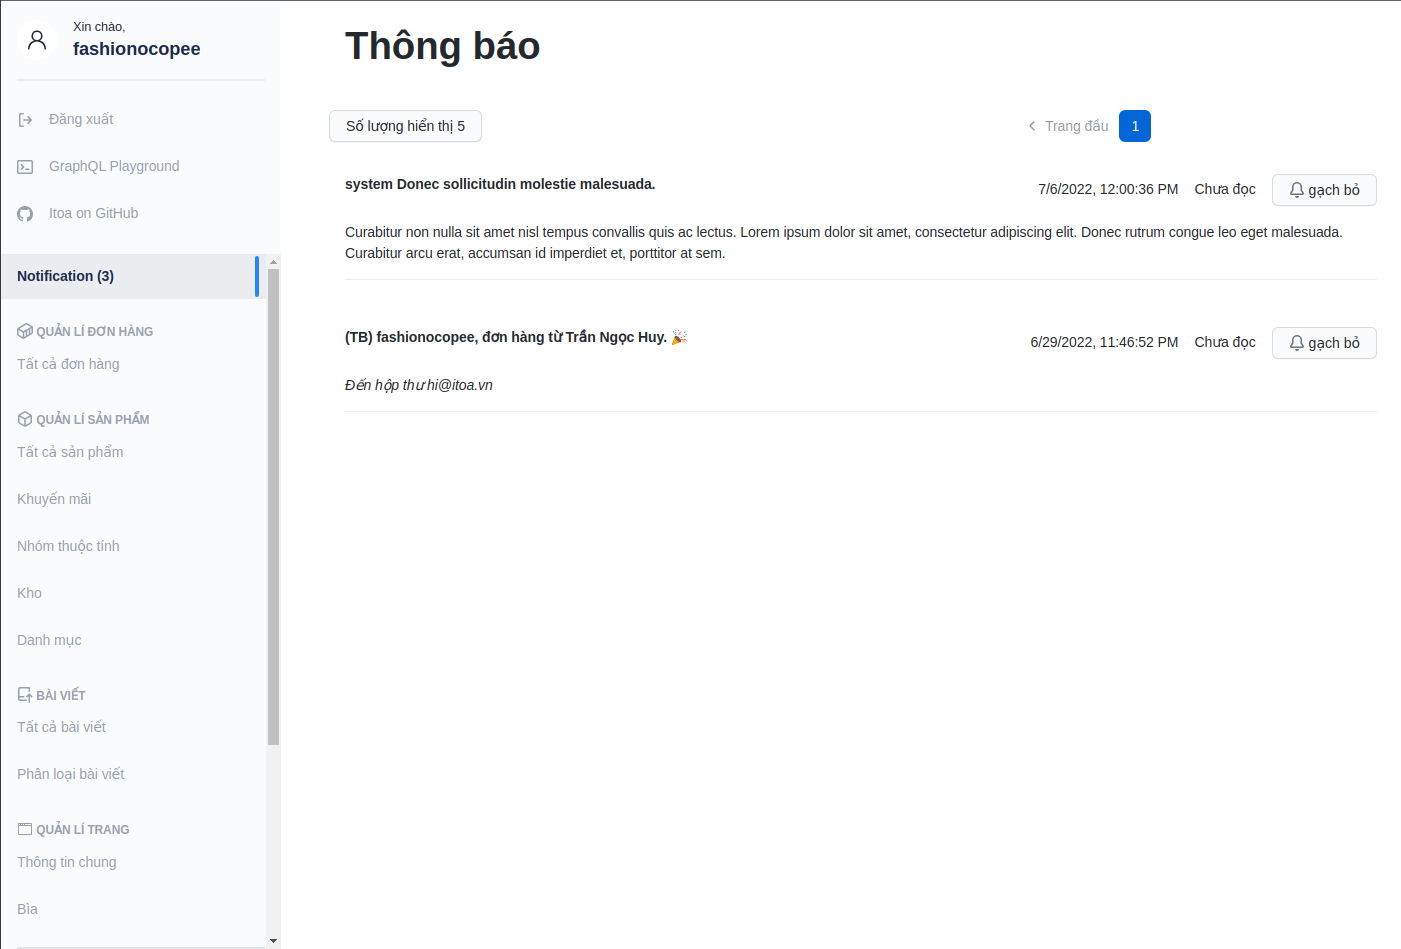
\includegraphics[width=\textwidth]{./results/notifications}
		\caption{Trang thông báo}
\justifying
Trang thông báo giúp cho nhà bán hàng hoặc nhà sản xuất kiểm tra hộp thư thông báo của mình. Đánh dấu các thông báo đã xem. Trang thông báo mặc định hiển thị ưu tiên các thông báo mới nhất chưa được xem.

Các thông báo đến địa chỉ thư điện tử của nhà bán hàng sẽ không được hiển thị nội dung mà thay vào đó. Thông báo chỉ hiển thị thông tin tiêu đề và ghi chú kiểm tra hộp thư.
\end{figure}
\clearpage
\subsubsection{Trang quản lí danh mục}
\FloatBarrier
\begin{figure}[!htbp]\fontsize{13px}{13px}\selectfont
\centering
		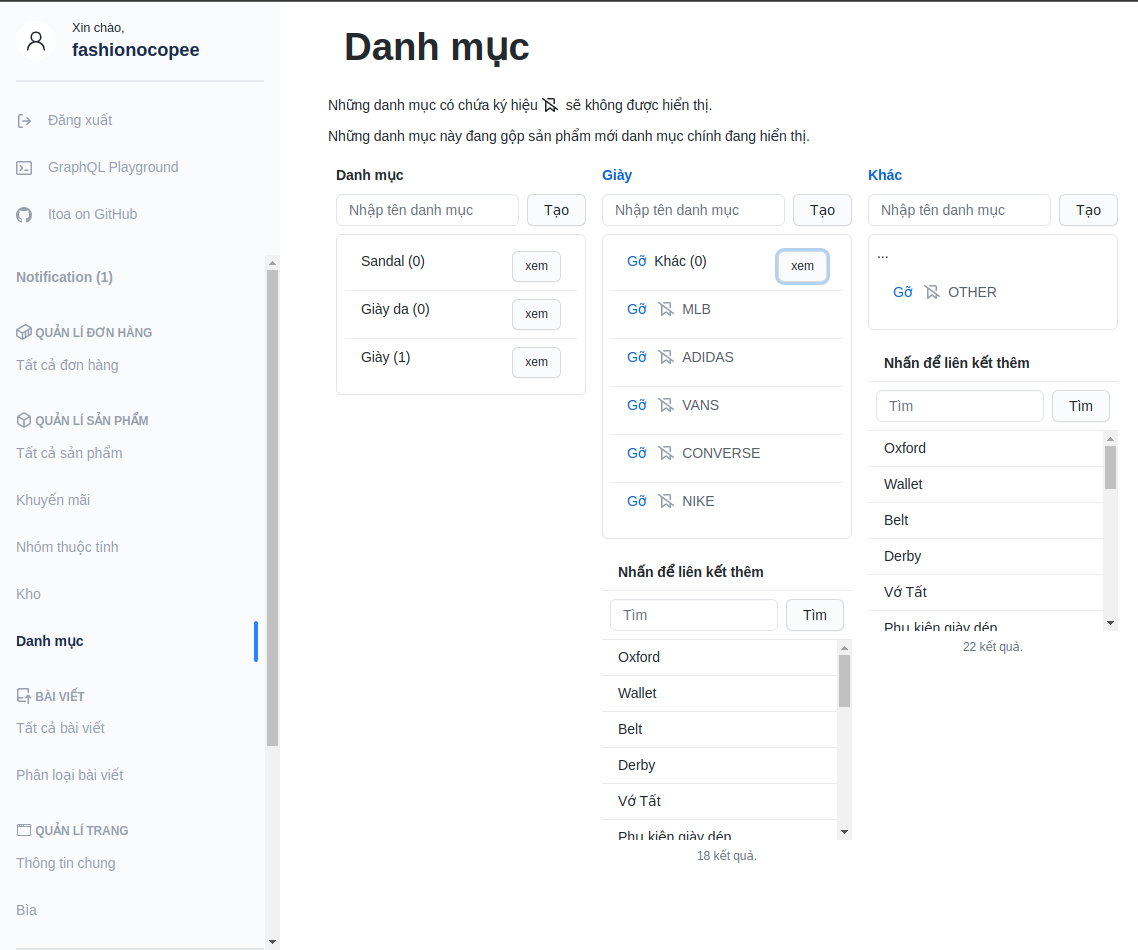
\includegraphics[width=\textwidth]{./results/categories}
		\caption{Trang quản lí danh mục}
\justifying
Quản lý danh mục giúp phân loại sản phẩm cho nhà sản xuất. Khi chia sẻ cho các nhà bán hàng. Danh mục sản phẩm có chức năng đánh dấu danh mục tương đương.

Nghĩa là đối với một nhà sản xuất hoặc nhà bán hàng. Họ luôn có cho mình cây danh mục do họ sở hữu. Và cũng là cây danh mục hiển thị chính trên trang.

Nhưng khi được chia sẻ sản phẩm, các sản phẩm được chia sẻ được liên kết với danh mục của nhà sản xuất. Và các danh mục ngoài nằm ngoài quyền quản lí của nhà bán hàng. Do vậy, tính năng danh mục tương đương đánh dấu các danh mục nào của nhà sản xuất là tương đương với danh mục của nhà bán hàng hiện tại. Sau khi đánh dấu tương được thì sản phẩm của nhà sản xuất, mặc dù nằm ngoài quyền quản lí của nhà bán hàng nhưng cũng có thể sắp xếp tìm kiếm bởi danh mục riêng của nhà bán hàng.
\end{figure}
\clearpage
\subsubsection{Trang quản lí tồn kho}
\FloatBarrier
\begin{figure}[!htbp]\fontsize{13px}{13px}\selectfont
	\centering
		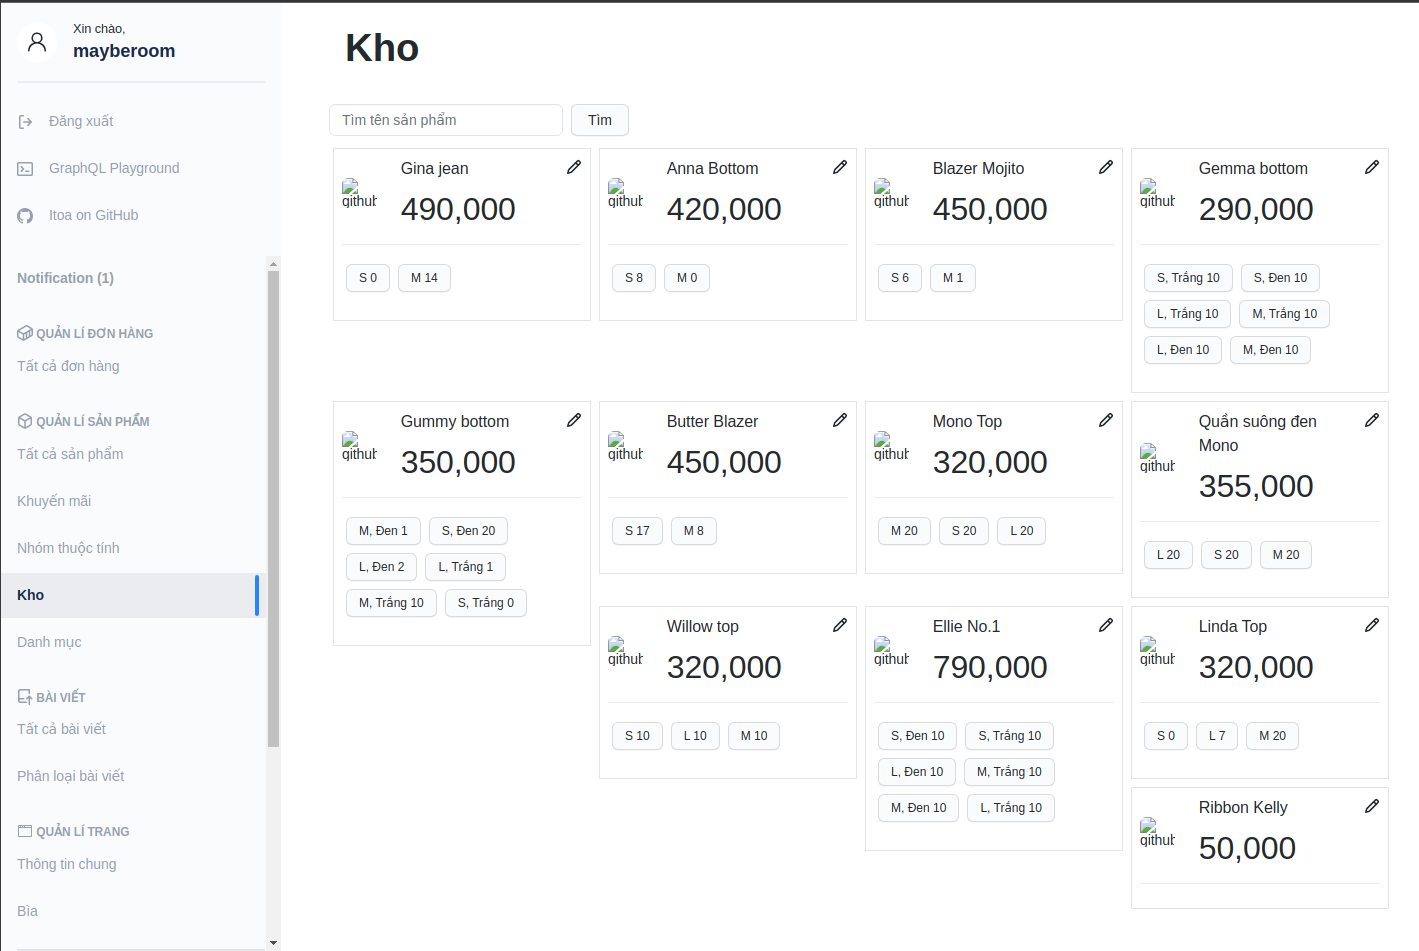
\includegraphics[width=\textwidth]{./results/stock}
		\caption{Trang quản lí tồn kho}
	\justifying
Quản lí có chức năng hiển thị tồn kho khi khách hàng chọn thuộc tính của sản phẩm. Ngăn chặn người dùng thêm nhiều hơn số tồn kho vào giỏ hàng hoặc mua sản phẩm hết hàng. Quản lí kho không bao gồm các chức năng tự động giảm số lượng trong kho khi đơn hàng sử lý thành công.
\end{figure}
\clearpage
\subsubsection{Trang quản lí thuộc tính}
\FloatBarrier
\begin{figure}[!htbp]\fontsize{13px}{13px}\selectfont
\centering
		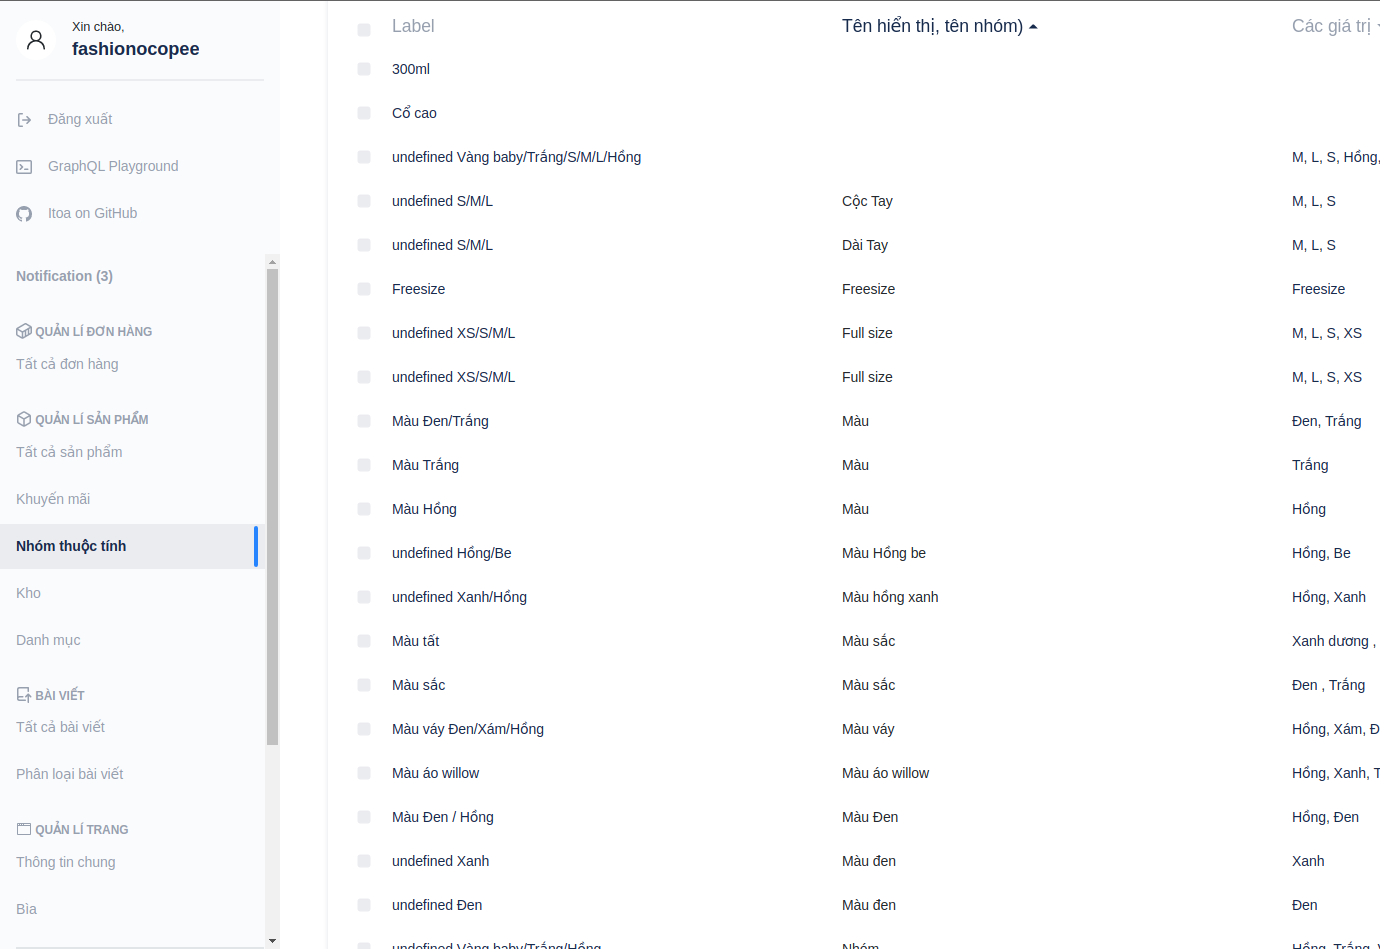
\includegraphics[width=\textwidth]{./results/attributes}
		\caption{Trang quản lí thuộc tính}
\justifying
Thuộc tính của một sản phẩm được định nghĩa là các phiên bản khác nhau của sản phẩm đó. Cùng một quy trình sản xuất hoặc cùng giá bán và chi phí sản xuất có thể cho là cùng một sản phẩm. Các thuộc tính của sản phẩm cũng được nhóm, quản lý kho và hình ảnh của thuộc tính đó. Ví dụ: kích thước, màu sắc. Cùng một sản phẩm giày nhưng khác màu sắc thì hình ảnh hiển thị cũng cần được lưu trữ và hiển thị trên trang.
\end{figure}
\clearpage
\subsubsection{Trang quản lí thông tin cửa hàng}
\FloatBarrier
\begin{figure}[!htbp]\fontsize{13px}{13px}\selectfont
\centering
		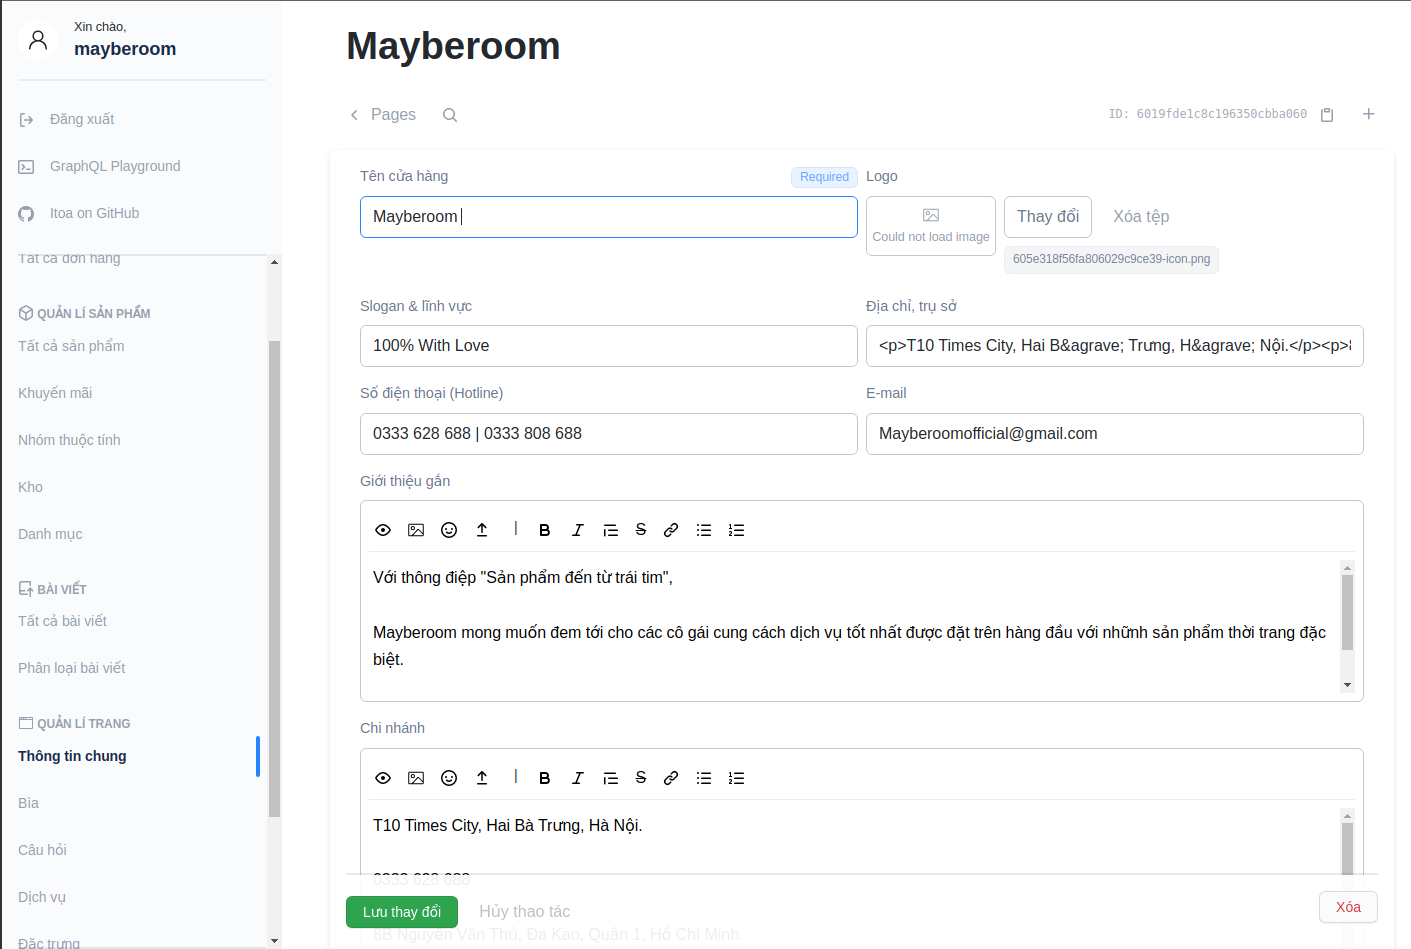
\includegraphics[width=\textwidth]{./results/store}
		\caption{Trang quản lí thông tin cửa hàng}
\justifying
Trang quản lý cửa hàng bao gồm các thông tin liên hệ cơ bản của nhà bán hàng. Các chính sách như thanh toán và vận chuyển.

Quản lí cửa hàng cũng bao gồm các thông tin thiết kế, tùy biến cá nhân hóa cho từng nhà bán hàng. Ví dụ như: Màu chủ đạo, lời chào,...
\end{figure}
\clearpage
\subsubsection{Trang quản lí mã giảm giá}
\FloatBarrier
\begin{figure}[!htbp]\fontsize{13px}{13px}\selectfont
\centering
		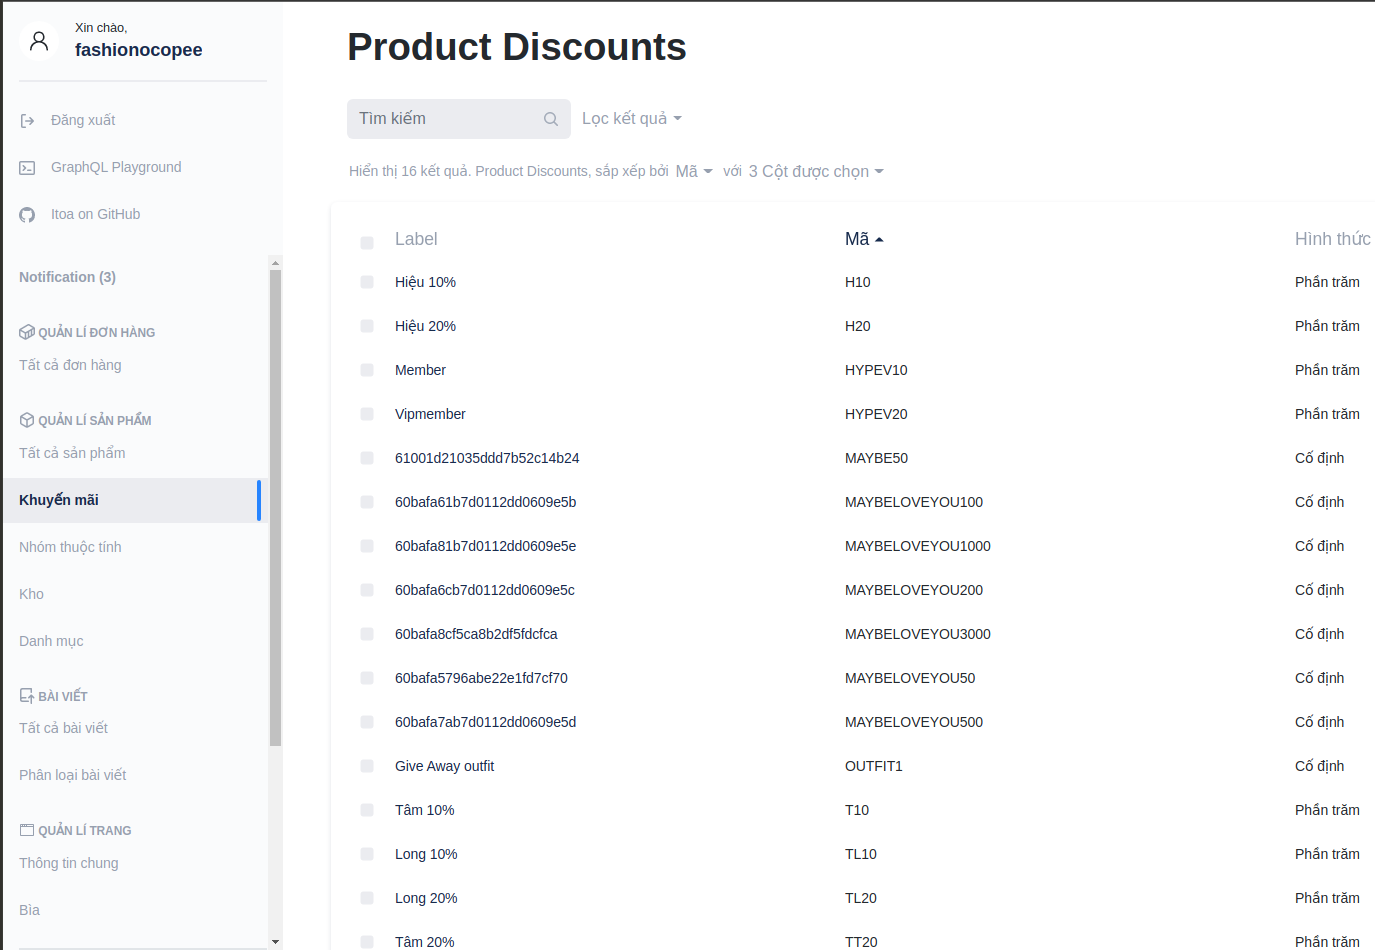
\includegraphics[width=\textwidth]{./results/discount}
		\caption{Trang quản lí mã giảm giá}
\justifying
	Trang quản lí mã khuyến mãi giúp người quản trị xem, sửa, xóa các mã khuyến mãi dựa theo phần trăm giảm. Hoặc theo giá cố định. Mã khuyến mãi cũng có thể đặt điều kiện tối thiểu để áp dụng mã giảm giá.
	
	Mã giảm giá của nhà sản xuất có thể được chia sẻ cho nhà bán hàng nhưng không thể sử dụng bởi một nhà sản xuất khác cũng cùng cung cấp sản phẩm cho nhà bán hàng.

	Mặc định mã giảm giá không thể truy cập bởi khách hàng, thông qua phiếu đặt hàng, mã giảm giá được nhập vào và kiểm tra trên hệ thống máy chủ.
\end{figure}
\clearpage
\subsubsection{Trang chủ sàn thương mại điện tử}
\FloatBarrier
\begin{figure}[!htbp]\fontsize{13px}{13px}\selectfont
\centering
		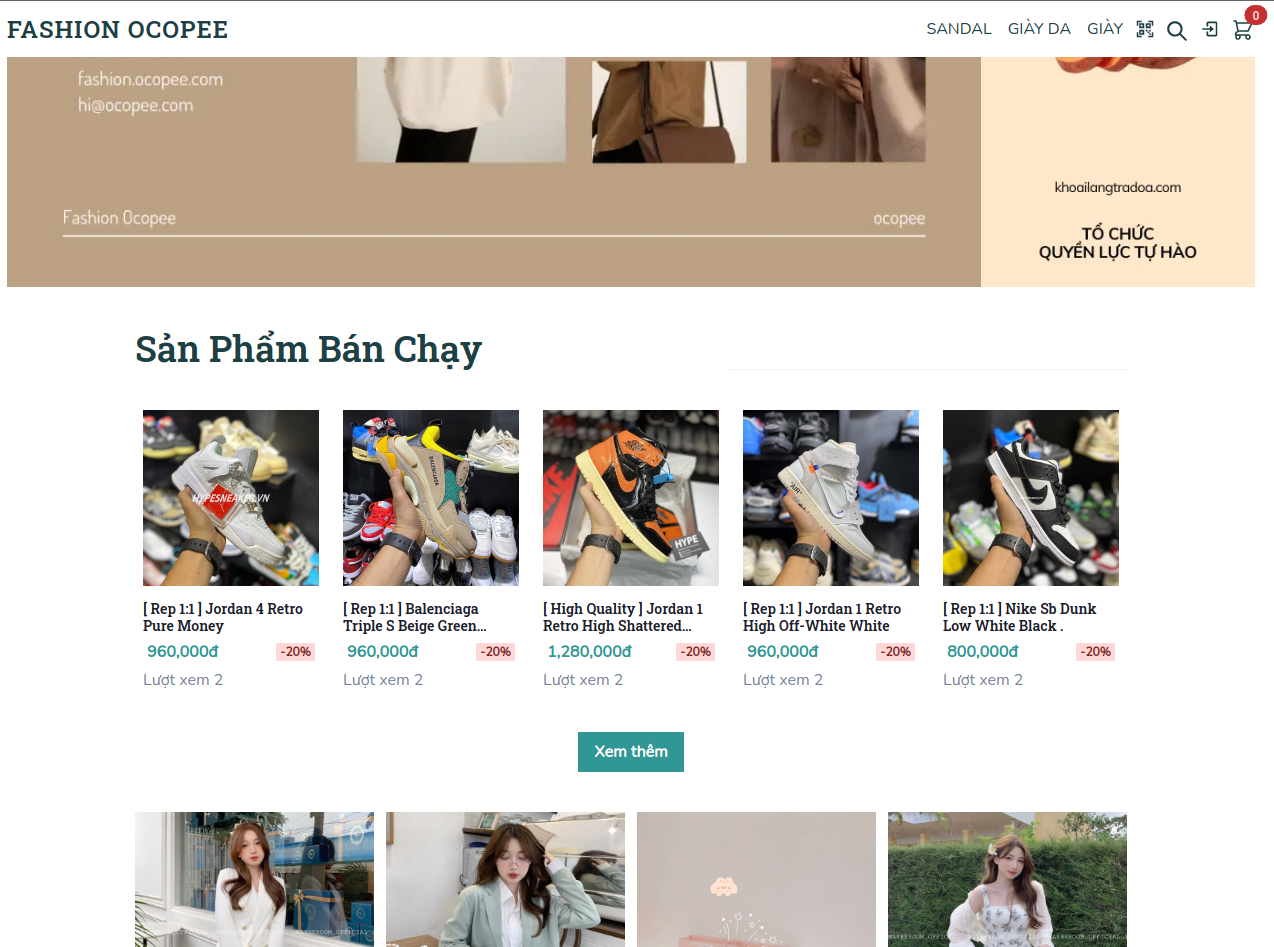
\includegraphics[width=\textwidth]{./results/homepage}
		\caption{Trang chủ sàn thương mại điện tử}
\justifying
Trang chủ sàn thương mại điện tử cho nhà bán hàng hiển thị các thông tin sản phẩm được chia sẻ cho sàn. Các hình ảnh quảng cáo. Điều hướng đến trang danh mục và chi tiết sản phẩm.
\end{figure}
\clearpage
\FloatBarrier
\begin{figure}[!htbp]\fontsize{13px}{13px}\selectfont
\centering
		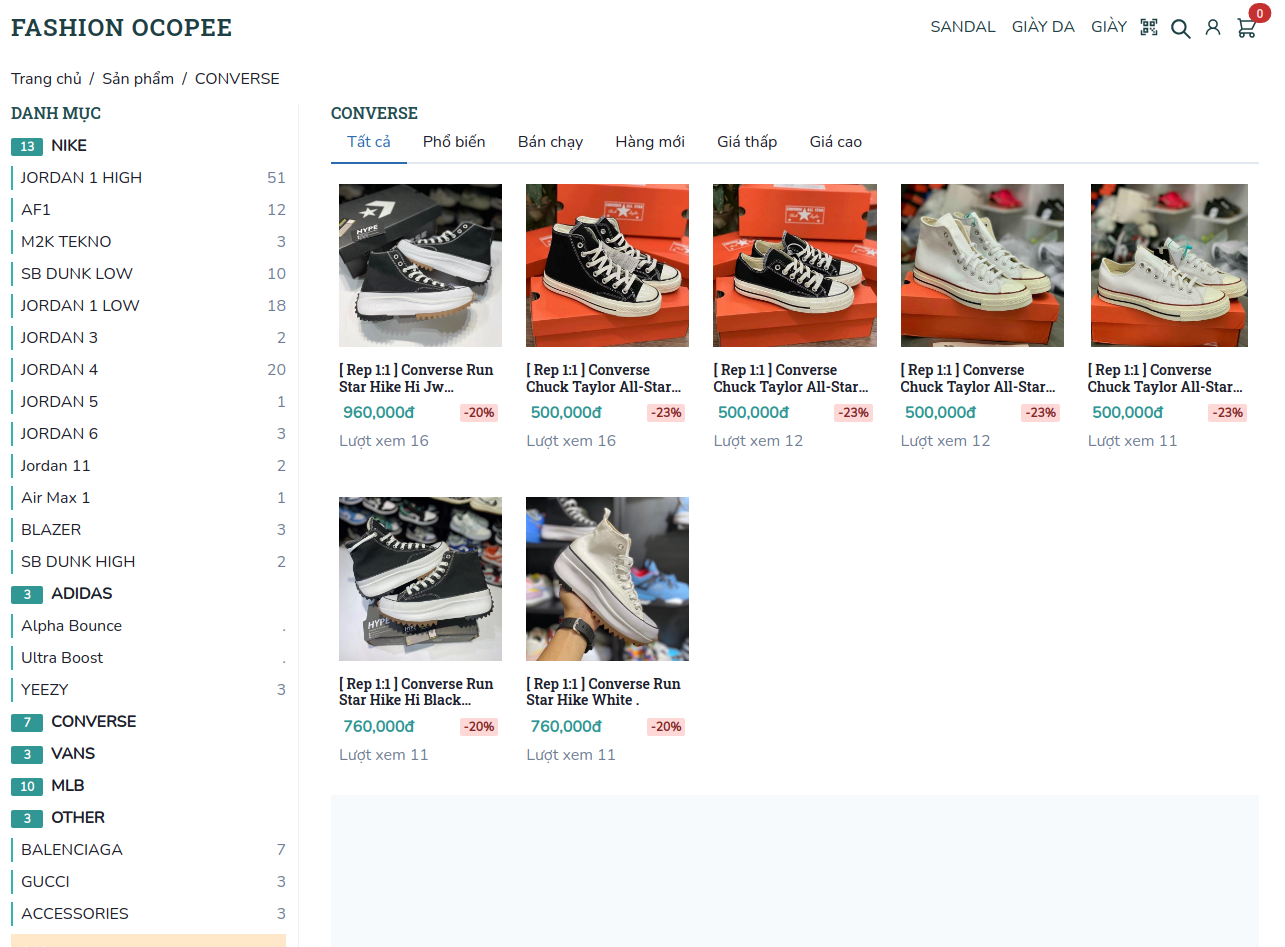
\includegraphics[width=\textwidth]{./results/categories-page}
		\caption{Trang duyệt xem sản phẩm}
\justifying
Trang duyệt xem hay còn gọi là trang trình bày sản phẩm, danh mục sản phẩm chung được quản lí bởi nhà bán hàng. Người dùng có thể xem sản phẩm theo danh mục, với các trạng thái như: bán chạy, phổ biến, hàng mới, giá thấp, giá cao... Nút xem thêm sản phẩm được thiết kế theo kiểu nối thêm sản phẩm thay vì lật trang.

\end{figure}
\clearpage
\FloatBarrier
\begin{figure}[!htbp]\fontsize{13px}{13px}\selectfont
\centering
		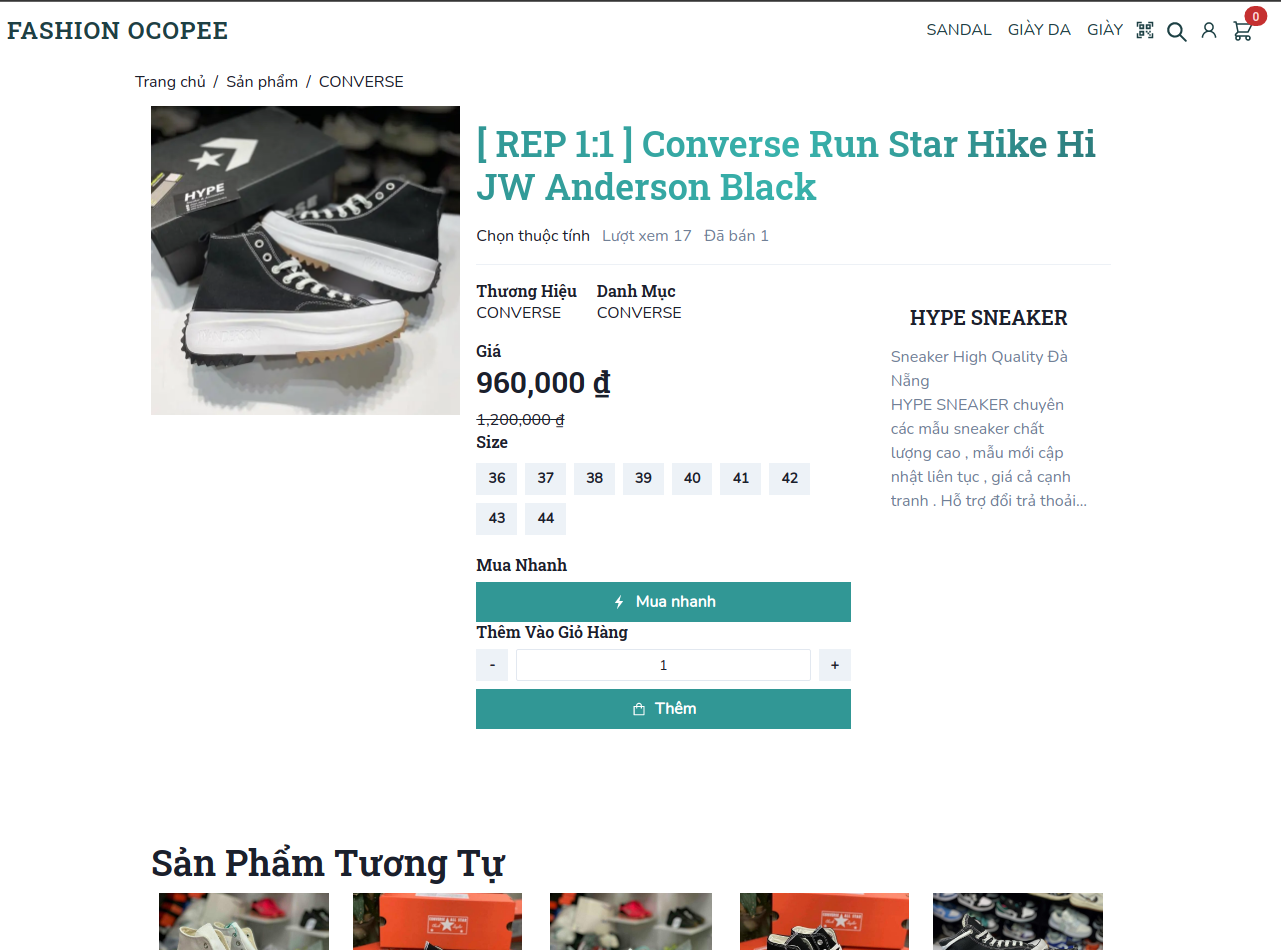
\includegraphics[width=\textwidth]{./results/product-page}
		\caption{Trang chi tiết sản phẩm}
\justifying
Trang chi tiết sản phẩm cho phép người mua hàng lựa chọn các thuộc tính của sản phẩm. Xem tồn kho của thuộc tính đó. Chức năng mua nhanh cho một sản phẩm duy nhất vào giỏ hàng và điều hướng đến trang thông tin đặt hàng. Chức năng thêm sẽ thêm số lượng sản phẩm tương ứng vào giỏ hàng. Bên cạnh thông tin chi tiết có hiển thị thông tin nhà cung cấp hoặc nhà sản xuất. Người dùng có thể đi đến không gian riêng của từng nhà sản xuất, trong trang chung hiện tại.
\end{figure}
\clearpage
\FloatBarrier
\begin{figure}[!htbp]\fontsize{13px}{13px}\selectfont
\centering
		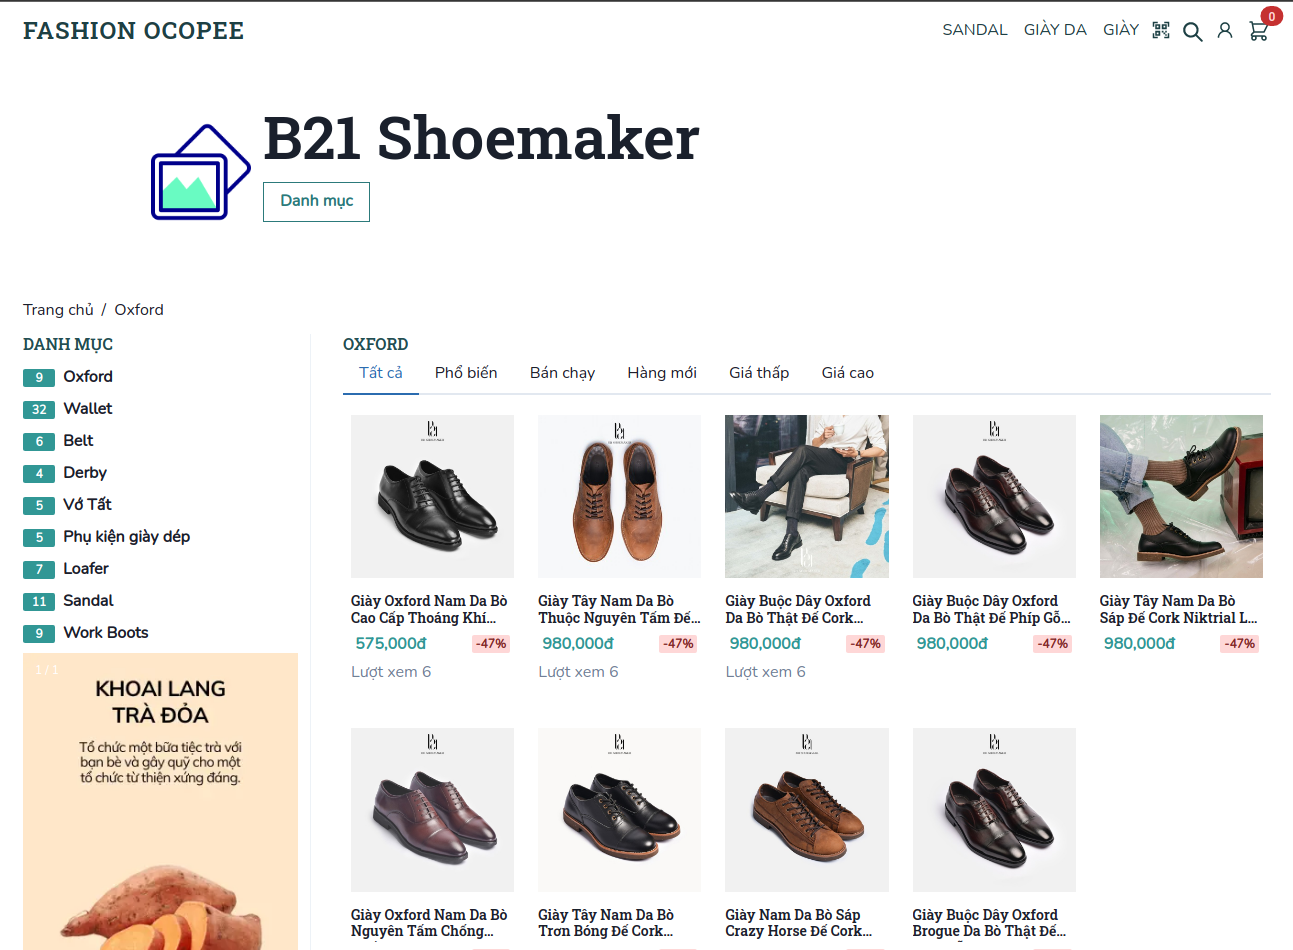
\includegraphics[width=\textwidth]{./results/store-page}
		\caption{Trang riêng của từng nhà sản xuất trên sàn}
\justifying
	Từng nhà sản xuất khi tham gia chia sẻ sản phẩm lên trang chung của nhà bán hàng cũng được xây dựng một không gian gian hàng riêng.
	Khác với trình bày sản phẩm chung, trang trình bày sản phẩm riêng cho từng nhà cung cấp, nhà sản xuất sử dụng danh mục sản phẩm được tạo ra bởi chính nhà sản xuất đó.
\end{figure}
\section{Đánh giá}
\subsection{Những vấn đề hạn chế}
Sau khi thực hiện đồ án em nhận thấy những vấn đề hạn chế sau:
\paragraph{micro-service} Kiến trúc này chỉ phù hợp cho các dự án lớn, nhiều nhóm làm việc với nhau. Chia thành service giúp các nhóm hoạt động độc lập với nhau. Các backlog được chia ra hoàn thành rồi quy nạp lại để khởi chạy toàn bộ hệ thống. Song song với việc phát hành phiên các mới của các service, việc duy trì các phiên bản ổn định cũ của service đó cũng khá tốn kém. Thường thì các hệ thống lớn duy trì hơn 10 phiên bản.

Việc sử dụng micro-service cho dự án nhỏ sẽ đẩy mức độ phức tạp lên quá mức cần thiết do phát chia cho hệ thống và cài đặt môi trường phát hành.

\paragraph{client side render} Việc giao tiếp thông qua API và kết xuất ứng dụng phía client giúp cho ứng dụng chạy mượt hơn. Nhưng đồng thời cũng làm tăng sự phụ thuộc vào interface giữa server và client. CSR không tối ưu đối với các máy chủ tìm kiếm hiện tại.

Thay vì mô hình thông thường toàn bộ trang được kết xuất và trả về một lần cho người dùng, CSR làm cho ứng dụng phân mảnh và cần nạp tải kết xuất nhiều lần mới dẫn đến kết quả cuối cùng.

\paragraph{search engine} Dự án vẫn chưa sử dụng search engine để tối ưu công việc tìm kiếm.

\paragraph{analysic} Hệ thống đo lường lưu lượng hoạt động tại các micro-service, các cầu nối chưa được phát triển đầy đủ. Điều này giúp quá trình nâng cao hiệu suất, cải thiên độ chịu tải của hệ thống trở nên khó khăn hơn.

\subsection{Hướng phát triển}

\paragraph{Mạng xã hội} Hiện tại hệ thống đã có tính năng kết bạn, cần phát triển thêm tính năng tương tác của mạng xã hội. Giúp không gian mua hàng trở nên sống động hơn. Cho phép khách hàng phản hồi về sản phẩm, đánh giá, trả lời bình luận. Xem các hoạt động của người khác ở thời điểm hiển tại.

\paragraph{Livestream} Tính năng livestream giúp cho nhà bán hàng xuất hiện lên tất cả các trang cho chia sẻ sản phẩm. Đồng thời cũng cần cam kết và kiểm duyệt nội dung của buổi livstreamstream.

\paragraph{Phân tích hành vi} Tính năng phân tích hành vi của người mua hàng, đánh giá mức độ ưu tiên hiển thị. Tạo nhiều tính năng giúp người dùng phản hồi nhanh về sản phẩm giúp nhà sản xuất cải thiện chất lượng.

\chapter*{KẾT LUẬN}
% size 14
\addcontentsline{toc}{chapter}{Kết luận}
%	Nội dung kết luận {Font: Time New Roman; thường; cỡ chữ: 13; dãn dòng: 1,3;căn lề: justified}
Đồ án đã vận dụng được các kiến thức nền tảng và ứng dụng các công cụ mới để phát triển hệ thống. Sau quá trình triển khai, em nhận thấy đồ án còn hạn chế ở khả năng tăng quy mô máy chủ để phục vụ cho lượng người dùng lớn. Đồng thời cũng chưa kiểm thử được hiệu suất của truy vấn dữ liêu khi lượng người dùng trở nên nhiều hơn.

Đồ án sẽ tiếp tục phát triển và phục vụ thực tế cho các doanh nghiệp sản xuất. Mở rộng thêm các tính năng phù hợp với nhu cầu doanh nghiệp. Đồng thời, các tính năng quan trọng cần được mở rộng phát triển trên nhiều nền tảng hệ điều hành.s

% Tham khảo
\bibliographystyle{alpha}
\bibliography{website}
\addcontentsline{toc}{chapter}{Tài liệu tham khảo}

\chapter*{PHỤ LỤC}
\pagenumbering{gobble}
\addcontentsline{toc}{chapter}{Phụ lục}

\chapter*{PHỤ LỤC}
\pagenumbering{gobble}
\addcontentsline{toc}{chapter}{Phụ lục}

\end{document}